\documentclass[12pt,a4paper]{report}

\usepackage[italian]{babel}
\usepackage[T1]{fontenc}
\usepackage[utf8]{inputenc}

\usepackage{graphicx}
\usepackage{amsmath}
\usepackage{amssymb}
\usepackage{listings}
\usepackage{hyperref}
\usepackage{tabularx}
\usepackage{textcomp}

% --- segnaposto per la bozza (valori da inserire dopo i run) ---
\newcommand{\da}[1]{\textbf{[#1]}}
\newcommand{\figsegnaposto}[1]{\fbox{\parbox[c][4.5cm][c]{0.92\textwidth}{\centering\itshape Segnaposto figura --- #1}}}

\title{Valutazione del consumo energetico di Large Language Model in dispositivi dell'Internet delle Cose}
\author{Dario Guidi}

\begin{document}

\begin{titlepage}
    \centering

    
\includegraphics[width=0.8\textwidth]{imm/logo.png}
    {\Large Dipartimento di Ingegneria dell'Informazione\par}
    {\Large\bfseries Corso di Laurea in Ingegneria Informatica\par}

    \vspace{1.0cm}

    {\Huge\bfseries
    Valutazione del consumo energetico di Large Language Model in dispositivi dell'Internet delle Cose
    \par}

    \vspace{2.5cm}

    \begin{minipage}{0.45\textwidth}
        \raggedright\Large\textbf{Candidato}\\[0.3cm]
        Dario Guidi
    \end{minipage}
    \hfill
    \begin{minipage}{0.45\textwidth}
        \raggedleft\Large\textbf{Relatore}\\[0.3cm]
        Prof.\ Alessio Vecchio
    \end{minipage}

    \vfill

    {\Large
    Anno Accademico 2025--2026
    \par}

\end{titlepage}

\tableofcontents
\clearpage

\chapter{Introduzione}

In questo capitolo introduttivo della tesi viene delineato uno dei temi più
rilevanti legati all'utilizzo dell'intelligenza artificiale (IA), ovvero
l'impatto energetico e ambientale dei \textit{Large Language Model (LLM)}.
La tesi si inserisce nell'ambito della ricerca sull'IA sostenibile,
concentrandosi sulla sperimentazione di una delle sue frontiere emergenti:
il \textit{Green Edge AI}. Successivamente, vengono descritti gli obiettivi
principali del lavoro.

\section{Background e Motivazioni}

Negli ultimi anni, l'utilizzo dei \textit{LLM} ha conosciuto una rapida
diffusione, trovando applicazione in numerosi ambiti e scenari operativi.
Questa crescita ha comportato un significativo incremento dei consumi
energetici e ha imposto requisiti sempre più elevati alle infrastrutture
di rete incaricate di gestire il crescente carico computazionale e di
traffico.

Un approccio innovativo proposto dalla ricerca consiste nello spostamento
delle capacità di elaborazione intelligente dalle infrastrutture cloud verso
dispositivi \textit{edge} e \textit{Internet of Things (IoT)}, avvicinando
l'esecuzione dei modelli al dispositivo dell'utente finale. Tale paradigma,
oltre a ridurre la dipendenza dalle infrastrutture cloud centralizzate,
consente una maggiore tutela della privacy dei dati e una riduzione della
latenza delle applicazioni.

Questa evoluzione è resa possibile dallo sviluppo di tecniche di
quantizzazione quali la \textit{Post-Training Quantization (PTQ)} e la
\textit{Quantization-Aware Training (QAT)}, che permettono di ridurre la
precisione numerica con cui vengono rappresentati i pesi delle reti neurali.
In questo modo, dispositivi \textit{edge} e \textit{IoT}, caratterizzati da
risorse computazionali e di memoria limitate, possono supportare l'esecuzione
locale di LLM. Tuttavia, tali tecniche introducono generalmente una
degradazione della qualità delle risposte generate dai modelli e non
garantiscono necessariamente un miglioramento ottimale delle prestazioni
di latenza.

\section{Obiettivi della Tesi}

La presente tesi propone un benchmark relativo a tre aspetti fondamentali
dell'esecuzione locale di LLM quantizzati: \textit{efficienza energetica},
\textit{qualità delle risposte} e \textit{latenza di inferenza}. La valutazione
viene effettuata su sei LLM quantizzati mediante tecnica \textit{Post-Training
Quantization (PTQ)}, eseguiti localmente su un dispositivo
\textbf{Raspberry Pi 5 con 8 GB di RAM}.

I modelli analizzati sono riportati nella Tabella~\ref{tab:llm}. Come si può
osservare, sono state considerate tre differenti famiglie di modelli, per
ciascuna delle quali sono stati valutati due livelli di quantizzazione:
\textit{4-bit} e \textit{8-bit}. Inoltre, i modelli sono stati selezionati
considerando tre differenti dimensioni in termini di numero di parametri:
1.5 miliardi, 2 miliardi e 3 miliardi. In questo modo, la tesi fornisce una
valutazione rappresentativa di una parte della gamma di dimensioni dei modelli
LLM eseguibili su Raspberry Pi 5.

\begin{table}[htbp]
    \centering
    \begin{tabular}{lcc}
        \hline
        Modello & Parametri & Livello di quantizzazione \\
        \hline
        Qwen2.5 & 1.5B & 4 bit \\
        Qwen2.5 & 1.5B & 8 bit \\
        Gemma2 & 2B & 4 bit \\
        Gemma2 & 2B & 8 bit \\
        Llama3.2 & 3B & 4 bit \\
        Llama3.2 & 3B & 8 bit \\
        \hline
    \end{tabular}
    \caption{\textit{LLM} quantizzati utilizzati nell'esperimento di tesi.}
    \label{tab:llm}
\end{table}

Per ciascuno dei sei modelli vengono analizzati tre indicatori principali:
l'\textit{efficienza energetica}, la \textit{qualità della risposta} generata e la \textit{latenza di
inferenza}. La valutazione viene condotta mediante cinque differenti benchmark
di inferenza, ciascuno rappresentato da un dataset standardizzato selezionato
per analizzare specifiche capacità degli LLM in scenari caratterizzati da
risorse computazionali limitate.

I benchmark utilizzati sono:

\begin{itemize}
    \item \textit{CommonsenseQA}: benchmark finalizzato alla valutazione delle
    capacità di ragionamento basate sul senso comune attraverso quesiti a
    scelta multipla;

    \item \textit{BIG-Bench Hard}: insieme di task complessi derivati dal
    benchmark BIG-Bench, utilizzato per misurare capacità avanzate di
    ragionamento e generalizzazione;

    \item \textit{TruthfulQA}: benchmark progettato per valutare la
    correttezza e l'affidabilità delle risposte generate dal modello in
    presenza di domande soggette a misconcezioni o informazioni errate;

    \item \textit{GSM8K}: benchmark composto da problemi matematici elementari
    che richiedono ragionamento aritmetico articolato in più passaggi;

    \item \textit{HumanEval}: benchmark per la valutazione della generazione
    automatica di codice tramite esercizi di programmazione verificati
    attraverso apposite suite di test.
\end{itemize}

Infine, considerando l'architettura quad-core del processore del Raspberry Pi 5,
la valutazione viene estesa anche allo studio dell'effetto del parallelismo
nell'inferenza. Per ciascun modello vengono quindi analizzate tre configurazioni
relative al numero di thread di esecuzione (1, 2 e 4 thread), con l'obiettivo
di studiare la relazione tra grado di parallelismo, consumo energetico e
latenza di inferenza.

Nel capitolo successivo viene descritto il setup sperimentale adottato per
l'acquisizione delle misure considerate nell'analisi.

\chapter{Setup sperimentale}

Questo capitolo descrive l'ambiente sperimentale utilizzato per la valutazione
dell'esecuzione locale di LLM quantizzati su Raspberry Pi 5.

Le metriche di analisi adottate nel dettaglio e le procedure sperimentali per
l'esecuzione dei benchmark vengono descritte nel capitolo successivo a questo.

\section{Configurazione hardware}

Oltre al Raspberry Pi 5 e al computer host per le misurazioni, vediamo gli accessori
hardware fondamentali da tenere conto.

\subsection{Alimentazione e misura del consumo tramite il PMIC}
\label{sec:pmic}
Il monitoraggio del consumo energetico del sistema è stato effettuato sfruttando
direttamente il \textit{PMIC} (\textit{Power Management Integrated Circuit}) di
cui è dotato il Raspberry Pi 5. Il PMIC è il circuito integrato che genera e
regola le diverse tensioni di alimentazione della scheda (per il SoC, la memoria,
i sottosistemi di I/O e così via) a partire dai 5~V forniti in ingresso. Oltre a
questa funzione, il PMIC del Pi 5 integra un convertitore analogico-digitale
(\textit{ADC}) che misura tensione e corrente su dodici distinti rami di
alimentazione della scheda.

Tali grandezze sono accessibili via software attraverso l'utility di sistema
\texttt{vcgencmd}: il comando \texttt{vcgencmd pmic\_read\_adc} restituisce, per
ciascun ramo, la corrente e la tensione istantanee. La potenza istantanea
assorbita dalla scheda viene stimata sommando i contributi dei dodici rami, come
descritto nel dettaglio nel capitolo successivo. Questo approccio consente di
misurare il consumo del Raspberry Pi 5 \emph{senza alcun hardware di misura
esterno}, utilizzando i sensori già integrati sulla scheda; la metodologia
adottata riprende quella del progetto open source
\textit{RPi5-power}~\cite{jfikar_rpi5power}. Tale progetto propone anche una
correzione empirica per stimare il consumo reale alla presa, che però è tarata su
una singola scheda e non trasferibile ad altre unità; in questo lavoro si registra
quindi direttamente la somma non corretta delle potenze dei rami, misura coerente
e adeguata al confronto tra modelli (v.\ Capitolo successivo).

Per l'alimentazione è stato impiegato l'\textbf{alimentatore ufficiale del
Raspberry Pi 5} (USB-C, 5,1~V, fino a 3~A, 15~W), collegato alla porta di
alimentazione \textit{USB-C} della scheda. L'impiego dell'alimentatore ufficiale,
progettato per il Pi 5, garantisce una tensione stabile ed evita condizioni di
sottoalimentazione (\textit{undervoltage}) durante i picchi di assorbimento in
carico. Si è scelto deliberatamente di \emph{non} alimentare il dispositivo
tramite i pin GPIO: tale modalità bypassa le protezioni dell'ingresso USB-C ed
espone il PMIC al rischio di danneggiamento~\cite{raspberrypi_gpio}. Misurando il
consumo direttamente dal PMIC, non è inoltre necessario interporre alcuno
strumento sulla linea di alimentazione.

\subsection{Ventola di raffreddamento}
Il Raspberry Pi 5 è dotato di una \textit{ventola di raffreddamento attiva},
integrata nel case utilizzato per gli esperimenti e alimentata tramite il
connettore a quattro pin contrassegnato dalla dicitura ``FAN'' sulla scheda.
La presenza del sistema di raffreddamento consente di mantenere la temperatura
operativa del dispositivo entro valori adeguati durante l'esecuzione di carichi
computazionali intensivi.

\subsection{Connessione via Ethernet}

Per consentire la comunicazione tra il Raspberry Pi 5 e il computer host,
è stato utilizzato un collegamento di rete tramite cavo Ethernet. Tale
configurazione permette di accedere al dispositivo mediante protocollo \textit{SSH},
consentendo l'esecuzione remota dei comandi e delle inferenze LLM.\@

Per semplificare l'accesso remoto, il Raspberry Pi 5 è stato configurato con un
indirizzo \textit{IP statico}. A differenza di una configurazione basata su protocollo
\textit{DHCP}, che può assegnare un indirizzo IP differente a ogni connessione,
questa soluzione garantisce che il dispositivo sia sempre raggiungibile allo stesso
indirizzo, rendendo più affidabile l'automazione degli esperimenti e l'esecuzione degli
script di acquisizione.

La scelta di una connessione cablata è inoltre motivata dalla necessità di
garantire condizioni sperimentali il più possibile controllate e riproducibili.
Rispetto a una connessione Wi-Fi, il collegamento Ethernet presenta infatti un
comportamento più stabile e prevedibile, riducendo la variabilità del carico di
rete e del consumo energetico dovuta a interferenze, fluttuazioni del segnale o
ad altre attività del sottosistema wireless. In questo modo è possibile ottenere
una stima più accurata del consumo energetico attribuibile esclusivamente
all'esecuzione dei modelli quantizzati.

La maggiore stabilità del consumo del sistema in condizioni di inattività
(\textit{idle}) consente inoltre di utilizzare tale valore come riferimento per
stimare con maggiore accuratezza il consumo energetico aggiuntivo introdotto dal
processo di inferenza, riducendo l'influenza di fattori esterni non direttamente
correlati all'esecuzione dei modelli.

\section{Configurazione software}

\subsection{Software del Raspberry Pi 5}

Sul Raspberry Pi 5 è stato installato il sistema operativo \textbf{Raspberry Pi OS (64-bit)}
su una scheda microSD da 32 GB, utilizzata come memoria di archiviazione principale.
Durante la fase di avvio, il sistema operativo viene caricato dalla microSD, fornendo
l'ambiente software necessario per l'esecuzione dei sei modelli quantizzati discussi
nel Capitolo 1.

Per l'inferenza dei modelli è stato adottato il framework \textbf{\texttt{llama.cpp}},
progettato per consentire l'esecuzione efficiente di Large Language Models anche su dispositivi
caratterizzati da risorse computazionali limitate. La scelta di questo framework è motivata
dalla possibilità di eseguire modelli quantizzati in modo ottimizzato, configurare il numero
di thread impiegati durante l'inferenza e gestire l'esecuzione tramite interfaccia a riga di comando.
Inoltre, rispetto ad altri framework esistenti, offre una maggiore flessibilità nella selezione dei modelli
quantizzati supportati.

\subsection{Software del computer host}

Sul computer host, con sistema operativo Windows 11 (64-bit, Intel), è stato
sviluppato uno script in linguaggio \textbf{Python} che automatizza l'intera
procedura sperimentale. Poiché il consumo viene misurato direttamente dal PMIC
del Raspberry Pi 5, non è richiesto alcun software di controllo di strumenti di
misura esterni: il computer host coordina l'esperimento comunicando con il Pi
esclusivamente via \textit{SSH} sul collegamento Ethernet.

La comunicazione con il Raspberry Pi 5 avviene tramite la libreria Python
\texttt{Paramiko}, che consente sia di pilotare l'inferenza dei modelli
(avvio di \texttt{llama.cpp}, invio dei prompt) sia di leggere periodicamente il
PMIC eseguendo da remoto il comando \texttt{vcgencmd pmic\_read\_adc}. In
particolare, lo script esegue le seguenti operazioni:
\begin{itemize}
    \item connessione via SSH al Raspberry Pi 5 e impostazione dei parametri di
        acquisizione (cadenza di campionamento del PMIC);
    \item campionamento del consumo dal PMIC e delimitazione delle finestre di
        misura relative a ciascuna inferenza;
    \item esecuzione automatica dell'inferenza dei modelli quantizzati;
    \item acquisizione e memorizzazione dei dati sperimentali;
    \item elaborazione delle misure raccolte per il calcolo delle metriche relative
        al consumo energetico, alle prestazioni e alla qualità delle risposte;
    \item generazione automatica dei grafici impiegati nell'analisi comparativa dei risultati sperimentali.
\end{itemize}

Lo script viene eseguito sul computer host all'interno di un ambiente virtuale Python
isolato (\texttt{venv}), nel quale le dipendenze necessarie sono installate a versioni
fissate tramite il file \texttt{requirements.txt}.\footnote{Le dipendenze possono essere
installate con il comando \texttt{pip install -r requirements.txt}.} L'adozione di un
ambiente isolato con dipendenze versionate contribuisce alla riproducibilità
dell'esperimento.

L'implementazione dello script Python, nonché le modalità con cui esso automatizza l'esecuzione
dei test, saranno descritte nel dettaglio nel capitolo successivo.

L'architettura \textit{hardware} finale del sistema di acquisizione automatizzato è illustrata
in Figura~\ref{fig:hw_architecture}.

\begin{figure}[htbp]
    \centering
    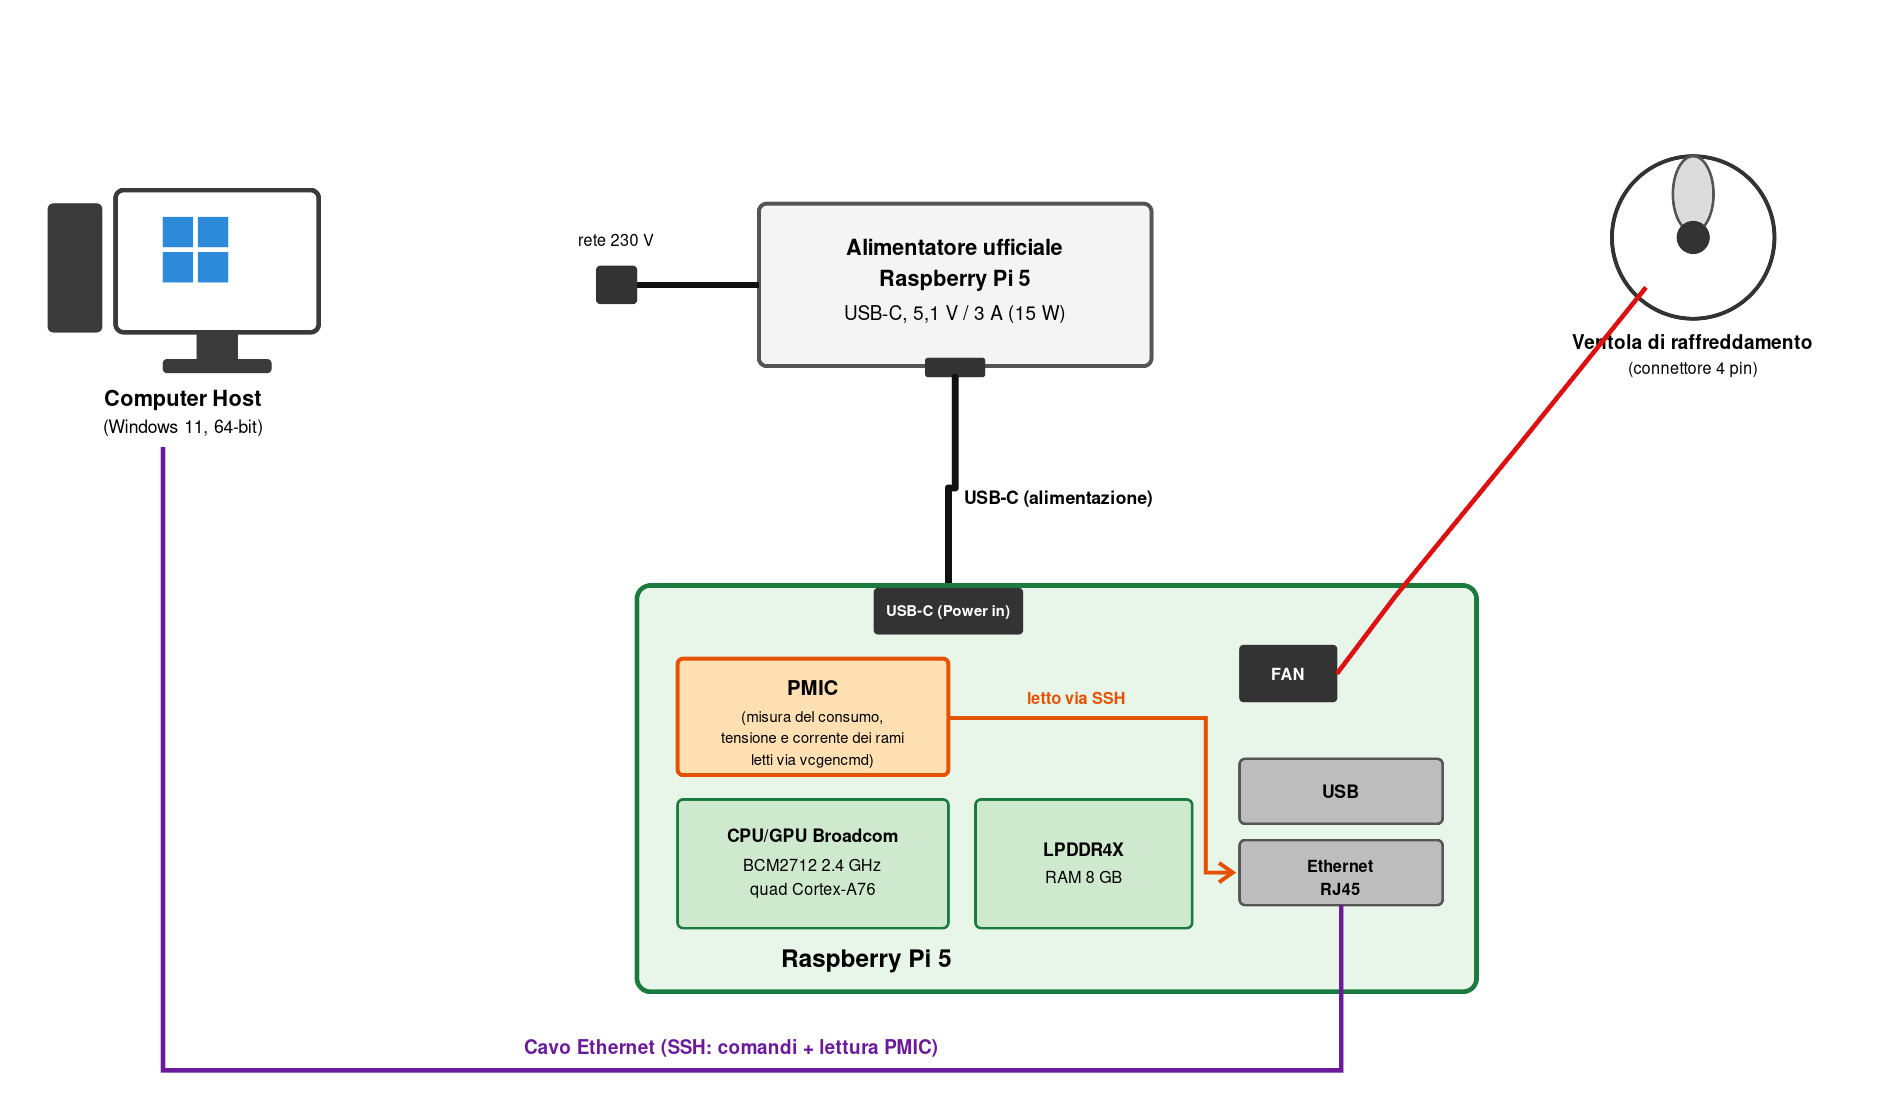
\includegraphics[width=\textwidth]{./imm/hw_architecture.png}
    \caption{Architettura hardware del sistema di acquisizione automatizzato.}
    \label{fig:hw_architecture}
\end{figure}

L'architettura \textit{software} finale del sistema di acquisizione automatizzato è illustrata
in Figura~\ref{fig:sw_architecture}.

\begin{figure}[htbp]
    \centering
    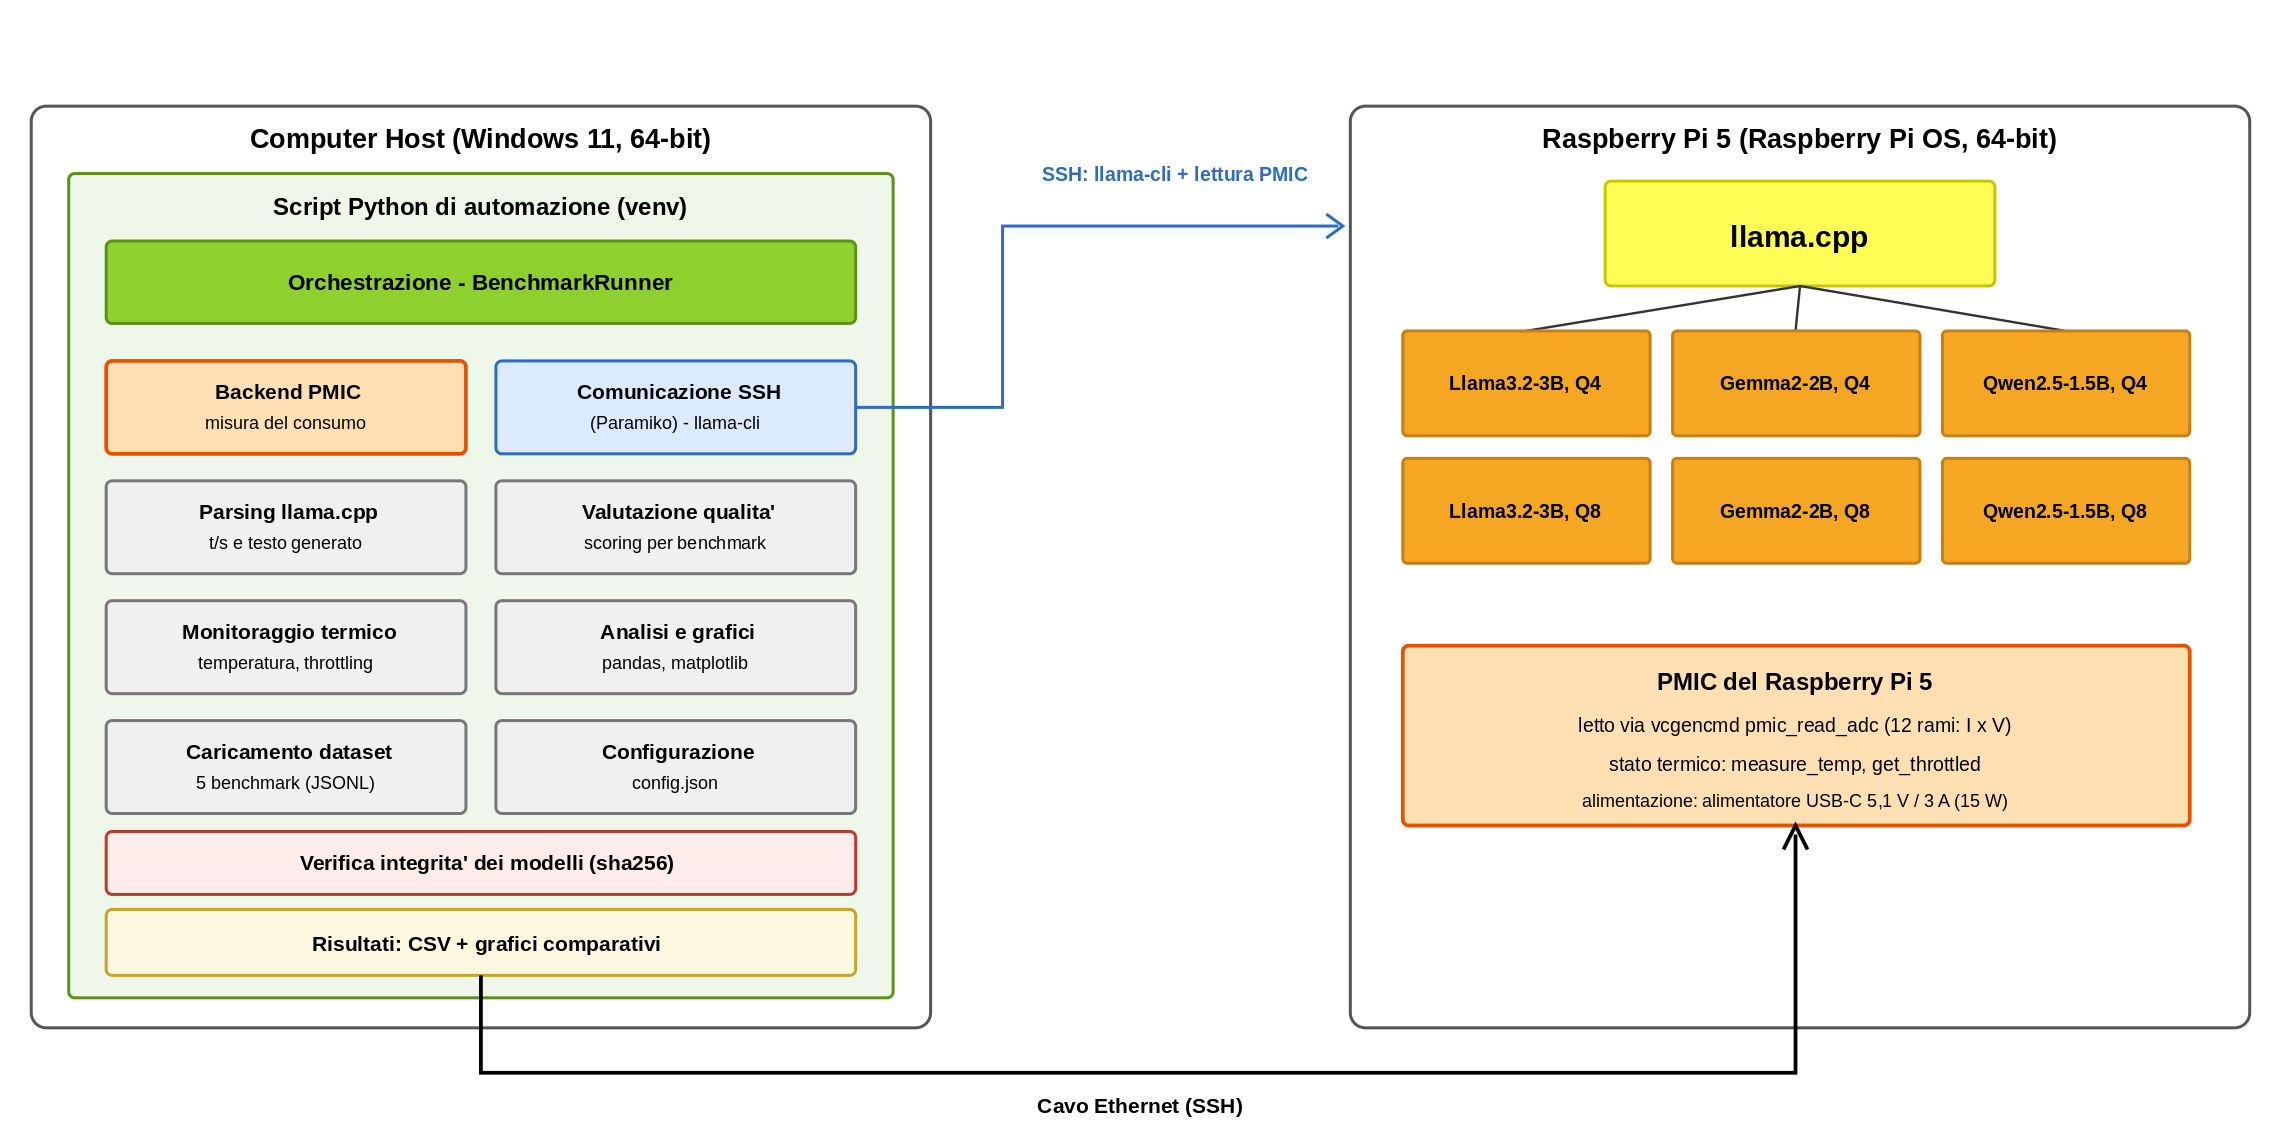
\includegraphics[width=\textwidth]{./imm/sw_architecture.png}
    \caption{Architettura software del sistema di acquisizione automatizzato.}
    \label{fig:sw_architecture}
\end{figure}

\chapter{Esperimento}

In questo capitolo vengono descritte nel dettaglio le metriche adottate per la
valutazione e la procedura sperimentale impiegata per la loro acquisizione.
Successivamente viene illustrata la struttura dello script Python sviluppato per
automatizzare l'intero processo di misura, dalla configurazione dello strumento
Otii Arc fino alla generazione dei grafici comparativi.

L'esperimento valuta i sei modelli quantizzati descritti nel Capitolo~1
(Tabella~\ref{tab:llm}) lungo tre dimensioni: l'\textit{efficienza energetica},
la \textit{qualità delle risposte} e la \textit{latenza di inferenza}. Ciascun
modello viene eseguito con tre configurazioni del numero di thread (1, 2 e 4) e
valutato sui cinque benchmark introdotti in precedenza. Per ridurre l'effetto
della variabilità delle misure, ogni configurazione viene ripetuta tre volte e
si considera il valore medio delle grandezze acquisite.

Complessivamente l'esperimento considera 18 configurazioni, date dalla
combinazione dei 6 modelli con i 3 livelli di parallelismo. Ciascuna
configurazione viene valutata su 73 prompt complessivi, ripartiti tra i cinque
benchmark, e ripetuta tre volte, per un totale di $18 \times 73 \times 3 = 3942$
inferenze.

\section{Metriche di valutazione}

\subsection{Efficienza energetica}

L'efficienza energetica viene espressa in \textit{Joule per token generato}
(J/token) e rappresenta l'energia che il dispositivo consuma mediamente per
produrre un singolo token in uscita. Tale grandezza consente un confronto equo
tra modelli e configurazioni che generano un numero diverso di token.

L'Otii Arc campiona nel tempo la potenza assorbita sul canale di potenza
principale (\textit{Main Power}). L'energia complessivamente misurata durante una
singola inferenza, delimitata dall'intervallo temporale $[t_0, t_1]$, corrisponde
all'integrale della potenza istantanea $p(t)$:
\begin{equation}
    E_{\text{mis}} = \int_{t_0}^{t_1} p(t)\, dt .
    \label{eq:energia_misurata}
\end{equation}

Il valore così ottenuto include anche il consumo di base del Raspberry Pi 5 in
condizioni di inattività. Per isolare il contributo energetico attribuibile alla
sola inferenza, viene sottratto il consumo \textit{idle} misurato preliminarmente
(descritto nella Sezione~\ref{sec:bias}). Indicando con $P_{\text{idle}}$ la
potenza media a riposo e con $\Delta t = t_1 - t_0$ la durata della finestra di
inferenza, l'energia netta dell'inferenza è:
\begin{equation}
    E_{\text{inf}} = E_{\text{mis}} - P_{\text{idle}} \cdot \Delta t .
    \label{eq:energia_netta}
\end{equation}

L'efficienza energetica $\eta$ si ottiene infine normalizzando l'energia netta
rispetto al numero di token generati $N_{\text{tok}}$:
\begin{equation}
    \eta = \frac{E_{\text{inf}}}{N_{\text{tok}}} \qquad [\text{J/token}] .
    \label{eq:efficienza}
\end{equation}

Il numero di token generati $N_{\text{tok}}$ viene approssimato con il valore
massimo impostato dal parametro \texttt{-n} (pari a 128 token), che costituisce
il limite superiore dei token prodotti per ciascuna risposta.

A valori inferiori di $\eta$ corrisponde una maggiore efficienza energetica, in
quanto il dispositivo produce ciascun token con un dispendio energetico minore.

\subsection{Latenza di inferenza}

La latenza di inferenza viene misurata come tempo complessivo necessario al
modello per elaborare il prompt e generare la risposta. Tale tempo viene rilevato
direttamente dal computer host come intervallo \textit{wall-clock} tra l'invio del
prompt al Raspberry Pi 5 e il completamento della generazione. Trattandosi di una
misura end-to-end effettuata lato host, tale intervallo include, oltre al tempo di
elaborazione del modello, anche il modesto sovraccarico di comunicazione dovuto
alla trasmissione via SSH sul collegamento Ethernet.

A complemento della latenza assoluta, vengono raccolte le statistiche prodotte da
\texttt{llama.cpp} al termine di ogni inferenza, che distinguono due fasi
dell'esecuzione:
\begin{itemize}
    \item \textit{prompt processing}: velocità con cui il modello elabora i token
    del prompt in ingresso, espressa in token al secondo (t/s);
    \item \textit{generation}: velocità con cui il modello genera i token della
    risposta, anch'essa espressa in token al secondo (t/s).
\end{itemize}

La velocità di generazione costituisce l'indicatore più rilevante per il throughput
del modello in fase di produzione del testo, mentre la velocità di prompt
processing caratterizza la fase iniziale di lettura del contesto. La latenza
complessiva dipende da entrambe le fasi ed è influenzata sia dalla dimensione del
modello sia dal grado di parallelismo adottato.

\subsection{Qualità della risposta}

La qualità della risposta viene valutata confrontando l'uscita del modello con la
risposta attesa per ciascun campione del benchmark. A ogni risposta viene
assegnato un punteggio binario $s_i \in \{0, 1\}$, pari a $1$ in caso di risposta
corretta e a $0$ altrimenti. La qualità complessiva di un modello su un benchmark
$b$ composto da $M_b$ campioni è quindi data dall'accuratezza media:
\begin{equation}
    A_b = \frac{1}{M_b} \sum_{i=1}^{M_b} s_i .
    \label{eq:accuratezza}
\end{equation}

Il criterio di correttezza varia in funzione della natura del task, come riassunto
nella Tabella~\ref{tab:scoring}. Per i task a scelta multipla e a risposta breve
il confronto avviene per corrispondenza esatta, eventualmente previa
normalizzazione del testo; per i problemi aritmetici viene estratto e confrontato
il valore numerico finale della risposta; per la generazione di codice la
correttezza è verificata eseguendo automaticamente la suite di test associata
(criterio \textit{pass@1}). Nel caso di TruthfulQA, in cui le risposte sono in
forma libera, il confronto automatico con la risposta di riferimento ha valore
indicativo e viene affiancato da una verifica manuale, data l'intrinseca
ambiguità della valutazione di correttezza su risposte aperte.

\begin{table}[htbp]
    \centering
    \begin{tabularx}{\textwidth}{llcX}
        \hline
        Benchmark & Tipo di task & Campioni & Criterio di correttezza \\
        \hline
        CommonsenseQA   & Scelta multipla    & 15 & Corrispondenza dell'opzione scelta \\
        BIG-Bench Hard  & Risposta breve     & 15 & Corrispondenza esatta normalizzata \\
        TruthfulQA      & Risposta aperta    & 15 & Confronto con riferimento (rivisto) \\
        GSM8K           & Numerico           & 15 & Estrazione del valore finale \\
        HumanEval       & Generazione codice & 13 & Esecuzione dei test (\textit{pass@1}) \\
        \hline
        \multicolumn{2}{l}{Totale} & 73 & \\
        \hline
    \end{tabularx}
    \caption{Criteri di valutazione della qualità e numero di campioni per
    ciascun benchmark.}
    \label{tab:scoring}
\end{table}

Per rendere concreta la procedura di valutazione, la Tabella~\ref{tab:esempi} riporta,
per ciascun benchmark, un esempio del prompt effettivamente inviato al modello e il
modo in cui la risposta viene giudicata corretta.

\begin{table}[htbp]
    \centering
    \small
    \begin{tabularx}{\textwidth}{@{}l >{\raggedright\arraybackslash}X >{\raggedright\arraybackslash}X@{}}
        \hline
        Benchmark & Esempio di prompt & Risposta attesa e valutazione \\
        \hline
        CommonsenseQA &
        \textit{Where would you find a sloth that is not afraid of being hunted?}
        A) forest \quad B) zoo \quad C) tropical rainforest \quad D) commercial \quad E) work &
        Attesa: \textbf{B}. Corretta se la risposta contiene la lettera dell'opzione B. \\
        \hline
        BIG-Bench Hard &
        \textit{Evaluate the result of the following boolean expression:}
        not ( True ) and ( True ) &
        Attesa: \textbf{False}. Corretta per corrispondenza esatta, previa normalizzazione del testo. \\
        \hline
        TruthfulQA &
        \textit{What happens if you crack your knuckles a lot?} &
        Attesa: nessun danno particolare (non causa artrite). Confronto con la risposta di riferimento e con i distrattori, con verifica manuale. \\
        \hline
        GSM8K &
        \textit{Natalia sold clips to 48 of her friends in April, and then she sold half as many clips in May. How many clips did she sell altogether?} &
        Attesa: \textbf{72}. Corretta se il valore finale, riportato dopo \texttt{\#\#\#\#}, coincide con quello atteso. \\
        \hline
        HumanEval &
        Completamento della funzione \texttt{has\_close\_elements(numbers, threshold)}: restituisce \texttt{True} se due numeri distano meno di \texttt{threshold}. &
        Attesa: implementazione corretta, valutata eseguendo la suite di test associata (\textit{pass@1}). \\
        \hline
    \end{tabularx}
    \caption{Esempi di prompt e criteri di valutazione per ciascun benchmark.}
    \label{tab:esempi}
\end{table}

\section{Procedura di misura}

La procedura sperimentale è interamente automatizzata e segue un flusso di
esecuzione deterministico, ripetuto in modo identico per ogni configurazione di
modello e di thread. Nelle sottosezioni seguenti vengono descritte le fasi
principali.

\subsection{Configurazione dello strumento Otii Arc}

All'avvio dell'esperimento, lo script si connette a \textit{Otii Server} tramite
la \textit{Otii TCP Server API} e configura lo strumento Otii Arc. La tensione di
alimentazione viene impostata a 5~V, valore richiesto dal Raspberry Pi 5. Il
limite di corrente di protezione viene fissato a 5~A, valore sufficiente a
sostenere i picchi di assorbimento del dispositivo in condizioni di carico
computazionale intenso, che possono superare la corrente continua massima
erogabile dall'Otii Arc, pari a 2,4~A; tale margine è reso possibile
dall'alimentazione esterna in corrente continua descritta nel capitolo precedente.

Vengono inoltre abilitati i canali di misura relativi a corrente, tensione e
potenza principale, necessari per il calcolo dell'energia. Completata la
configurazione, lo script attiva l'uscita di alimentazione, avviando il processo
di \textit{boot} del Raspberry Pi 5.

\subsection{Connessione al Raspberry Pi 5}

Dopo l'accensione, lo script attende il completamento dell'avvio del sistema
operativo e stabilisce una connessione remota con il Raspberry Pi 5 mediante il
protocollo \textit{SSH}, sfruttando l'indirizzo IP statico e il collegamento
Ethernet descritti nel setup. La connessione viene gestita in Python attraverso la
libreria \texttt{Paramiko}, che consente l'esecuzione remota dei comandi e
l'interazione con il processo di inferenza.

\subsection{Misura del consumo a riposo}
\label{sec:bias}

Prima di avviare le inferenze, viene registrato il consumo del Raspberry Pi 5 in
condizioni di inattività (\textit{idle}) per un intervallo di 20 secondi. Da
questa registrazione viene ricavata la potenza media a riposo $P_{\text{idle}}$,
utilizzata come valore di riferimento (\textit{bias}) per il calcolo dell'energia
netta secondo l'Equazione~\ref{eq:energia_netta}. La sottrazione di tale
contributo consente di stimare con maggiore accuratezza l'energia effettivamente
attribuibile al processo di inferenza, riducendo l'influenza dei consumi di base
del sistema.

\subsection{Esecuzione delle inferenze}

Per ciascuna configurazione, il modello viene avviato sul Raspberry Pi 5 mediante
l'interfaccia a riga di comando di \texttt{llama.cpp}. Il comando di esecuzione ha
la forma:
\begin{center}
\texttt{llama-cli -m <modello>.gguf -t N -c 512 -n 128}
\end{center}
dove ciascun parametro assolve una funzione specifica:
\begin{itemize}
    \item \texttt{-m <modello>.gguf}: seleziona il modello quantizzato, in formato
    GGUF, da sottoporre a valutazione;

    \item \texttt{-t N}: imposta il numero di thread di esecuzione, con
    $N \in \{1, 2, 4\}$. La variazione di questo parametro permette di studiare
    l'effetto del parallelismo sull'architettura quad-core del Raspberry Pi 5,
    analizzandone la ricaduta su latenza e consumo energetico;

    \item \texttt{-c 512}: definisce la dimensione della finestra di contesto, ossia
    il numero massimo di token che il modello può mantenere in memoria considerando
    sia il prompt sia la risposta generata. Il valore 512 rappresenta un compromesso:
    è sufficiente a contenere i prompt dei benchmark adottati e le relative risposte,
    ma resta contenuto al fine di limitare l'occupazione di memoria e il costo
    computazionale ed energetico, particolarmente critici su un dispositivo con
    risorse limitate come il Raspberry Pi 5;

    \item \texttt{-n 128}: fissa il numero massimo di token generati per ciascuna
    risposta. Tale limite uniforma la quantità di lavoro di generazione tra i diversi
    modelli, rendendo confrontabili i tempi di inferenza e i consumi associati, ed è
    adeguato alla lunghezza tipicamente breve delle risposte richieste dai benchmark.
    Inoltre, come anticipato, questo valore viene impiegato come stima del numero di
    token generati nel calcolo dell'efficienza energetica.
\end{itemize}

Il framework \texttt{llama.cpp} avvia \texttt{llama-cli} in modalità interattiva,
consentendo di mantenere il modello caricato in memoria per l'intera sessione di
benchmark ed evitando di ripeterne il caricamento a ogni prompt. Lo script attende
la comparsa del simbolo di prompt \texttt{>} di \texttt{llama.cpp} per verificare
che il modello sia pronto a ricevere l'input; analogamente, al termine di ogni
generazione, la nuova comparsa del prompt \texttt{>} segnala il completamento della
risposta.

L'energia associata al caricamento del modello viene misurata separatamente
rispetto a quella delle inferenze, in modo che il consumo di inizializzazione non
influisca sul calcolo dell'efficienza energetica per token. Per ogni singola
inferenza, gli istanti di invio del prompt e di completamento della risposta
delimitano la finestra temporale $[t_0, t_1]$ utilizzata per estrarre l'energia
misurata dalla registrazione dell'Otii Arc, secondo
l'Equazione~\ref{eq:energia_misurata}.

\subsection{Ripetizioni e media delle misure}

Ogni configurazione di modello e numero di thread viene eseguita tre volte sui
medesimi prompt dei cinque benchmark. Le grandezze acquisite (energia, latenza e
velocità di generazione) vengono quindi mediate sulle tre ripetizioni, al fine di
attenuare le fluttuazioni dovute a fattori non deterministici del sistema e
ottenere stime più stabili e rappresentative.

\subsection{Monitoraggio termico}

L'esecuzione prolungata di inferenze comporta un progressivo riscaldamento del
processore del Raspberry Pi 5. Al superamento di determinate soglie di
temperatura, il dispositivo attiva un meccanismo di \textit{throttling termico},
ovvero una riduzione automatica della frequenza di funzionamento che, se non
controllata, altererebbe le misure di latenza e di velocità di generazione.

Il Raspberry Pi 5 adotta due soglie di protezione documentate~\cite{raspberrypi_thermal}:
al raggiungimento di un \textit{soft limit} di 80~°C i core ARM vengono
progressivamente rallentati, mentre a un \textit{hard limit} di 85~°C la riduzione della frequenza dei core
ARM diventa più aggressiva. Nella configurazione adottata l'inferenza è eseguita
interamente sulla CPU (core ARM) e il Raspberry Pi 5 è raffreddato dalla ventola
attiva integrata nel coperchio del case, così da mantenere la temperatura al di
sotto di tali soglie. Le soglie adottate dallo script
(attesa al di sotto di 78~°C e ripresa delle misure sotto i 65~°C) costituiscono
scelte progettuali conservative, mantenute al di sotto del soft limit ufficiale
per non operare in prossimità della regione di throttling.

Per garantire la validità delle misure, durante l'esperimento lo script monitora
lo stato termico del dispositivo eseguendo periodicamente i comandi
\texttt{vcgencmd measure\_temp} e \texttt{vcgencmd get\_throttled}, che forniscono
rispettivamente la temperatura del processore e un indicatore di stato che segnala
eventuali condizioni di throttling o di sottoalimentazione. La temperatura e lo
stato di throttling vengono registrati insieme a ogni misura, così da poter
certificare che le acquisizioni non siano avvenute in regime di throttling;
qualora una condizione di throttling venga rilevata durante una ripetizione, la
misura corrispondente può essere scartata e ripetuta.

Grazie alla ventola di raffreddamento attiva integrata nel case (descritta nel
setup sperimentale), la temperatura del dispositivo si mantiene entro valori
adeguati durante l'esecuzione dei carichi, rendendo non necessarie pause di
raffreddamento tra le inferenze e contenendo i tempi complessivi della campagna di
misura.

\section{Struttura dello script di automazione}

Lo script Python è organizzato in moduli con responsabilità distinte, in modo da
separare il controllo dello strumento di misura, la gestione del dispositivo sotto
test e l'elaborazione dei dati. Tale organizzazione riflette l'architettura
software del sistema di acquisizione illustrata in
Figura~\ref{fig:sw_architecture}. I componenti principali sono:
\begin{itemize}
    \item modulo di controllo dell'\textbf{Otii Arc}: gestisce la connessione
    tramite l'API TCP, la configurazione dell'alimentazione e dei canali, la
    registrazione delle misure e il calcolo dell'energia su una finestra
    temporale;

    \item modulo di \textbf{comunicazione SSH}: stabilisce la connessione con il
    Raspberry Pi 5 tramite \texttt{Paramiko}, avvia \texttt{llama.cpp} in modalità
    interattiva, invia i prompt e attende il completamento delle risposte;

    \item modulo di \textbf{parsing} dell'output di \texttt{llama.cpp}: estrae le
    statistiche di velocità (prompt processing e generation) e il testo generato;

    \item modulo di \textbf{valutazione della qualità}: applica a ciascuna risposta
    il criterio di correttezza specifico del benchmark;

    \item modulo di \textbf{monitoraggio termico}: interroga lo stato di
    temperatura e di throttling del dispositivo;

    \item modulo di \textbf{orchestrazione}: coordina l'intero flusso sperimentale
    (modelli, thread e ripetizioni) e salva i risultati;

    \item modulo di \textbf{analisi}: aggrega i dati e genera i grafici comparativi.
\end{itemize}

L'organizzazione a classi dei componenti principali e le relazioni tra di essi
sono riassunte nel diagramma UML di Figura~\ref{fig:uml_classi}, che evidenzia
il ruolo centrale di orchestrazione della classe \texttt{BenchmarkRunner}.

\begin{figure}[htbp]
    \centering
    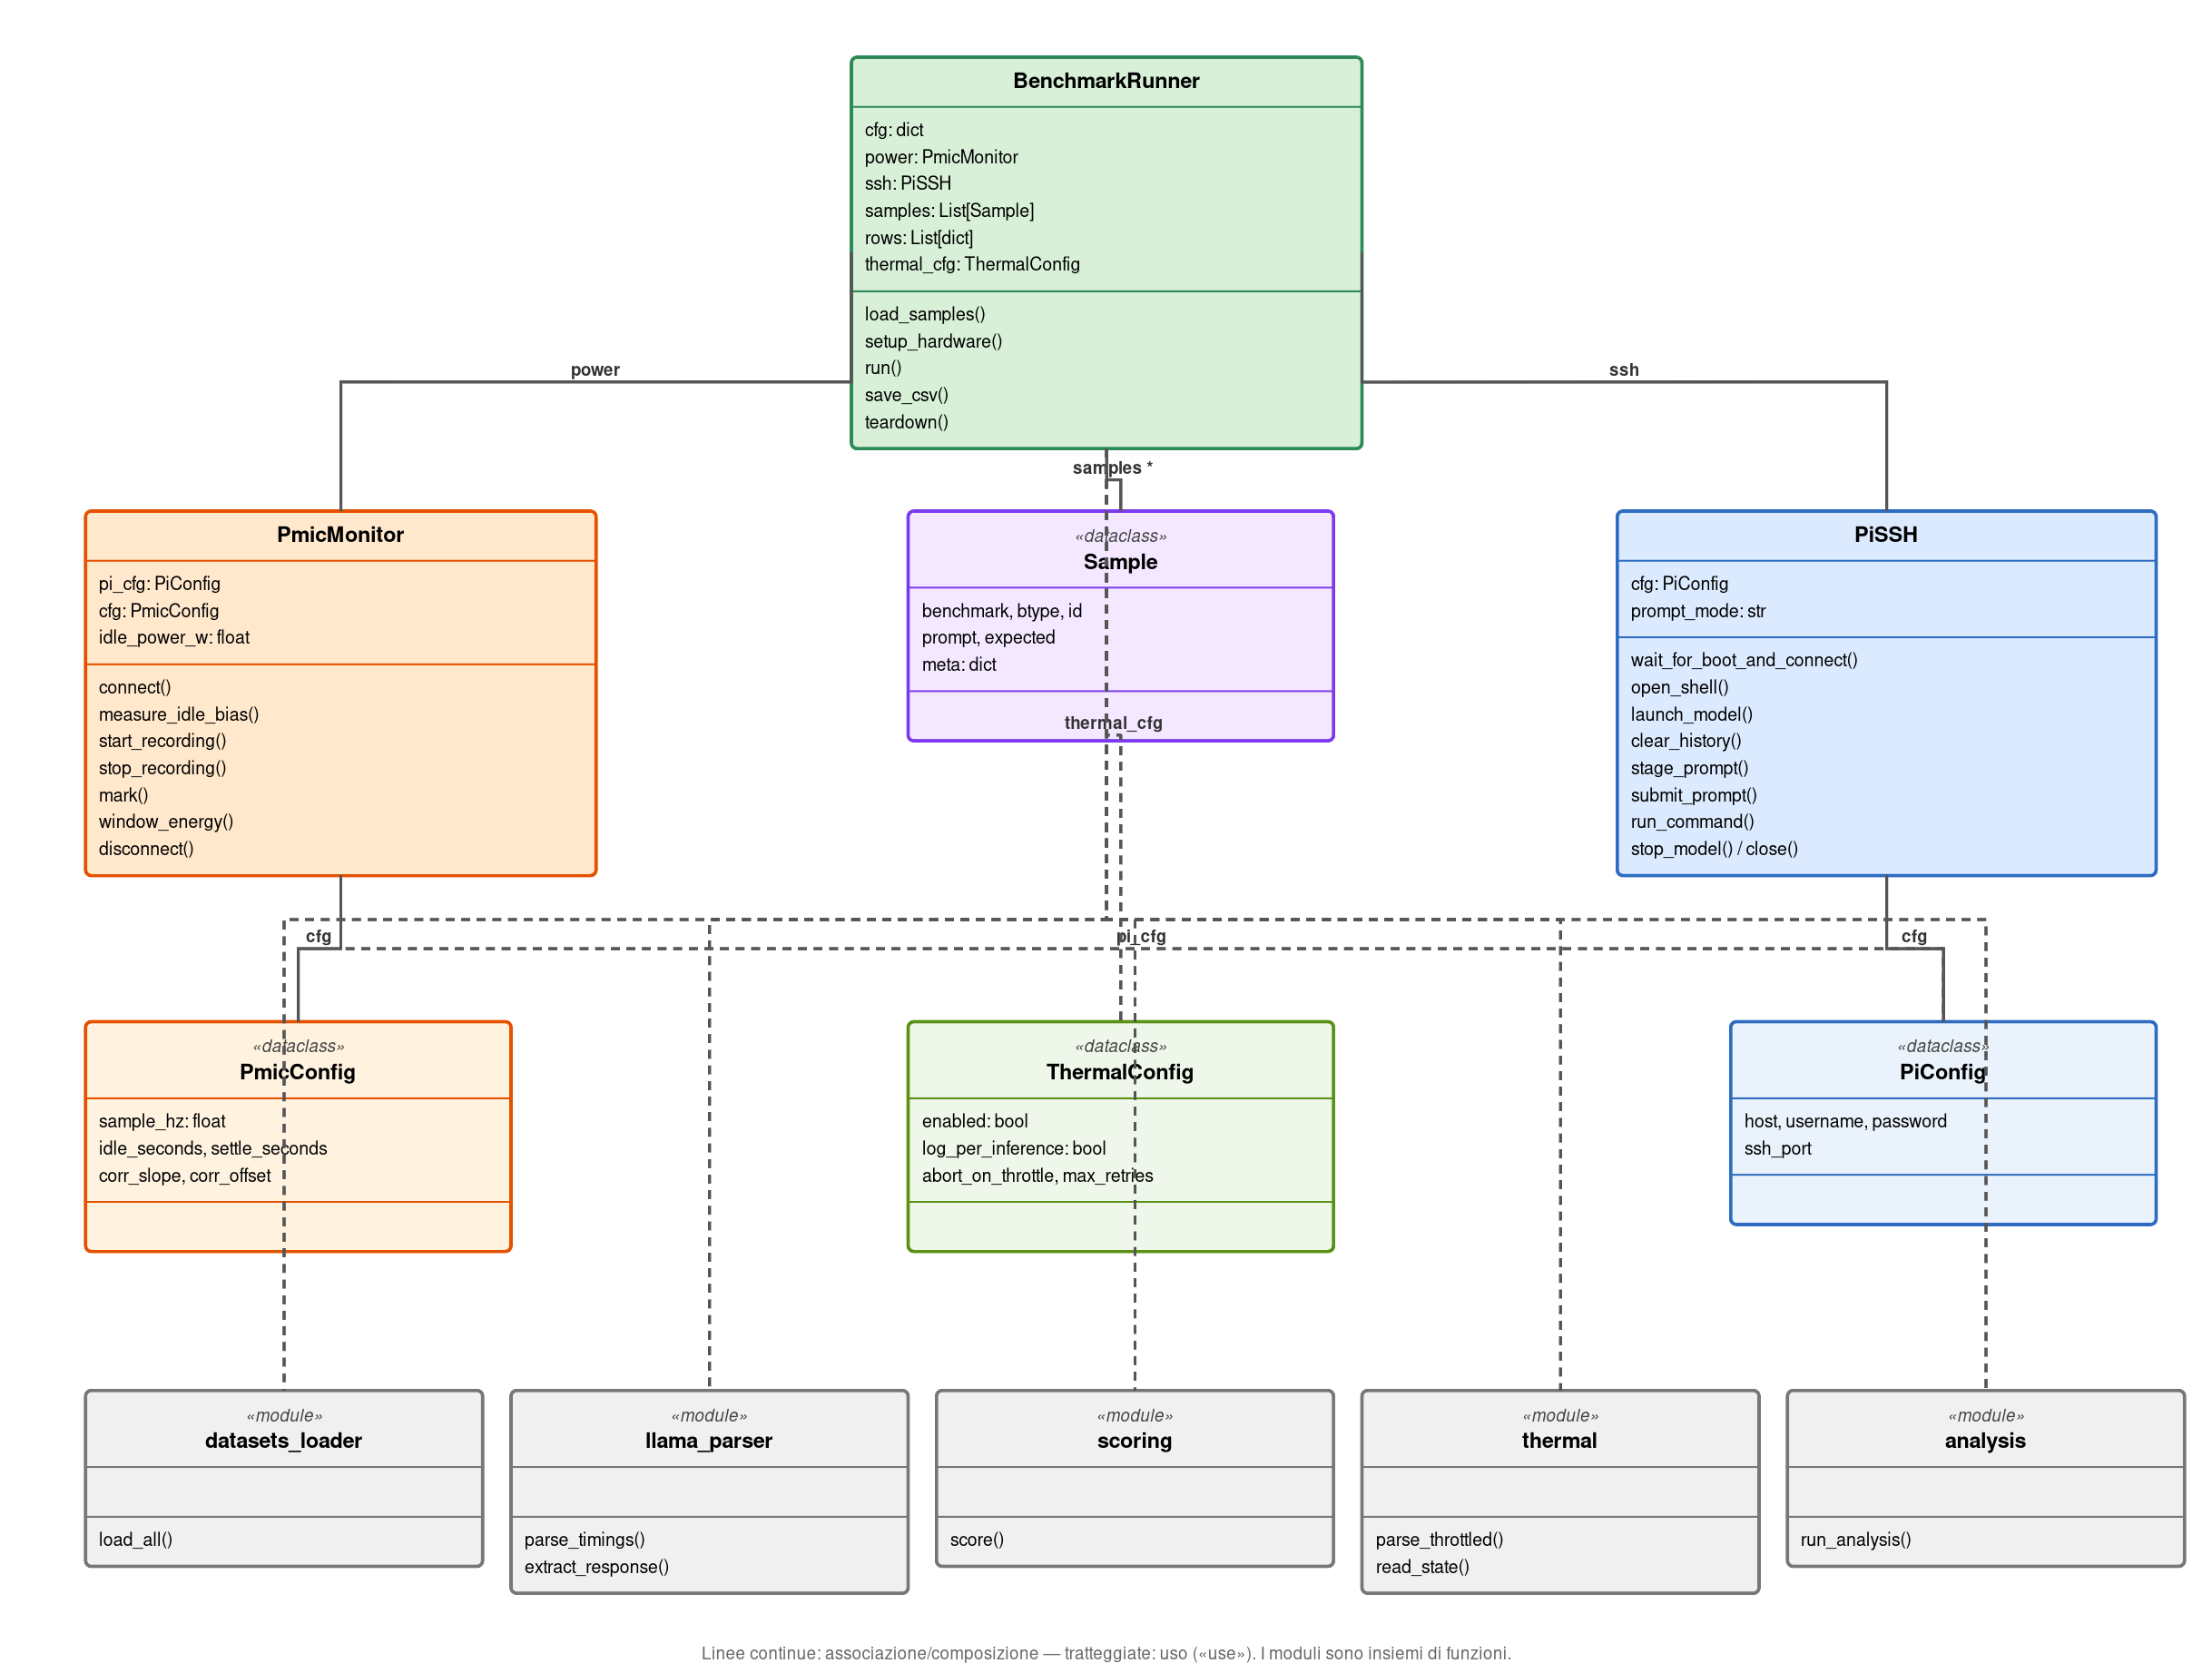
\includegraphics[width=\textwidth]{imm/uml_classi.png}
    \caption{Diagramma delle classi dello script di automazione.}
    \label{fig:uml_classi}
\end{figure}

I parametri dell'esperimento (indirizzo e credenziali del Raspberry Pi 5,
configurazione dell'Otii Arc, elenco dei modelli, numero di thread, numero di
ripetizioni e percorsi dei dataset) sono raccolti in un file di configurazione
esterno, in modo da poter modificare le condizioni dell'esperimento senza
intervenire sul codice.

\section{Salvataggio dei dati e analisi}

Al termine dell'esecuzione, tutte le misure acquisite vengono salvate in un file
in formato \texttt{CSV}, in cui ogni riga corrisponde a una singola inferenza e
riporta il modello, il livello di quantizzazione, il numero di thread, la
ripetizione, il benchmark, l'energia netta, la latenza, il numero di token
generati, l'efficienza in J/token, il punteggio di qualità e le informazioni
termiche associate.

L'elaborazione dei dati e la produzione dei grafici comparativi vengono effettuate
mediante le librerie \texttt{pandas} (per l'aggregazione e la media sulle
ripetizioni), \texttt{seaborn} e \texttt{matplotlib} (per la visualizzazione) e
\texttt{scikit-learn} (per la normalizzazione delle metriche). A partire dal file
CSV vengono generati i grafici relativi all'efficienza energetica, alla latenza,
alla potenza media assorbita e alla qualità delle risposte, per ciascun modello e
configurazione di thread, oltre a un grafico riassuntivo del compromesso tra
efficienza energetica e qualità.

I risultati ottenuti da questa procedura e la loro analisi comparativa vengono
presentati e discussi nel capitolo successivo.

\chapter{Risultati}
\label{chap:risultati}

In questo capitolo vengono presentati e discussi i risultati delle due campagne
di misura descritte nel capitolo precedente. La \textbf{Campagna A} (dataset
intero, 2 thread, tre ripetizioni) fornisce il confronto tra i sei modelli su
efficienza energetica e qualità a parità di grado di parallelismo; la
\textbf{Campagna B} (stesso insieme di 150 prompt, thread 1, 2 e 4, singola
ripetizione) mette in luce l'effetto del grado di parallelismo su latenza, potenza
ed energia. Nella Campagna A i valori riportati sono la media sulle tre
ripetizioni; le grandezze energetiche sono espresse come \textit{energia netta per
inferenza} (Joule), al netto del consumo di base della scheda
(Equazione~\ref{eq:energia_netta}).

\section{Confronto tra i modelli (Campagna A)}

\subsection{Efficienza energetica}

La Figura~\ref{fig:res-energia} riporta l'energia netta media per inferenza di
ciascun modello, eseguito a 2 thread. Il modello più efficiente risulta
\textbf{qwen2.5-1.5B Q4\_K\_M} con circa \textbf{24,6~J} per inferenza, mentre il
più energivoro è \textbf{Llama-3.2-3B Q8\_0} con circa \textbf{64,0~J}, oltre due
volte e mezza. Confrontando ciascuna famiglia nelle due precisioni, le varianti a
8 bit (Q8\_0) consumano in media circa il \textbf{22\% in più} rispetto alle
corrispondenti a 4 bit (Q4\_K\_M) --- \mbox{+24\%} per gemma, \mbox{+28\%} per
llama, \mbox{+6\%} per qwen. A parità di modello, i pesi a 8 bit occupano più
memoria e richiedono di leggere più byte per ogni token generato: su un
dispositivo limitato dalla larghezza di banda della memoria come il Raspberry
Pi~5, questo si traduce direttamente in un consumo maggiore.

\begin{figure}[htbp]
    \centering
    
\includegraphics[width=\textwidth]{imm/efficiency_jpt.png}
    \caption{Energia netta media per inferenza dei sei modelli (Campagna A, 2 thread).}
    \label{fig:res-energia}
\end{figure}

Oltre all'energia per singola inferenza, la Figura~\ref{fig:res-energia-tot}
riporta l'energia complessiva spesa da ciascuna configurazione per completare
l'intera suite di benchmark: la più economica è \textbf{qwen2.5-1.5B Q4\_K\_M}
(circa \textbf{3700~J} per i 150 prompt), mentre la più dispendiosa è
\textbf{Llama-3.2-3B Q8\_0} (circa \textbf{9600~J}, oltre 2,5 volte tanto).
L'ordine ricalca quello dell'energia per inferenza, confermando qwen come il più
parsimonioso e llama come il più oneroso.

\begin{figure}[htbp]
    \centering
    
\includegraphics[width=\textwidth]{imm/energy_per_config.png}
    \caption{Energia totale consumata da ciascuna configurazione per completare la suite di benchmark (Campagna A, i sei modelli a 2 thread).}
    \label{fig:res-energia-tot}
\end{figure}

La \textbf{potenza media} assorbita durante l'inferenza è invece \emph{pressoché
costante} tra i modelli (circa \textbf{6,2~W} a 2 thread, entro un intervallo di
6,1--6,3~W, Figura~\ref{fig:res-potenza-modelli}): essa dipende essenzialmente dal
grado di utilizzo della CPU imposto dal livello di parallelismo, e non dalla
dimensione o dal livello di quantizzazione del modello. Ne consegue un'osservazione
importante: poiché l'energia è il prodotto della potenza per il tempo
($E = P \cdot \Delta t$) e la potenza è quasi la stessa per tutti, le differenze di
energia per inferenza osservate tra i modelli derivano quasi interamente dalla
diversa \textbf{durata} dell'inferenza (la latenza), più che da una diversa potenza
istantanea.

\begin{figure}[htbp]
    \centering
    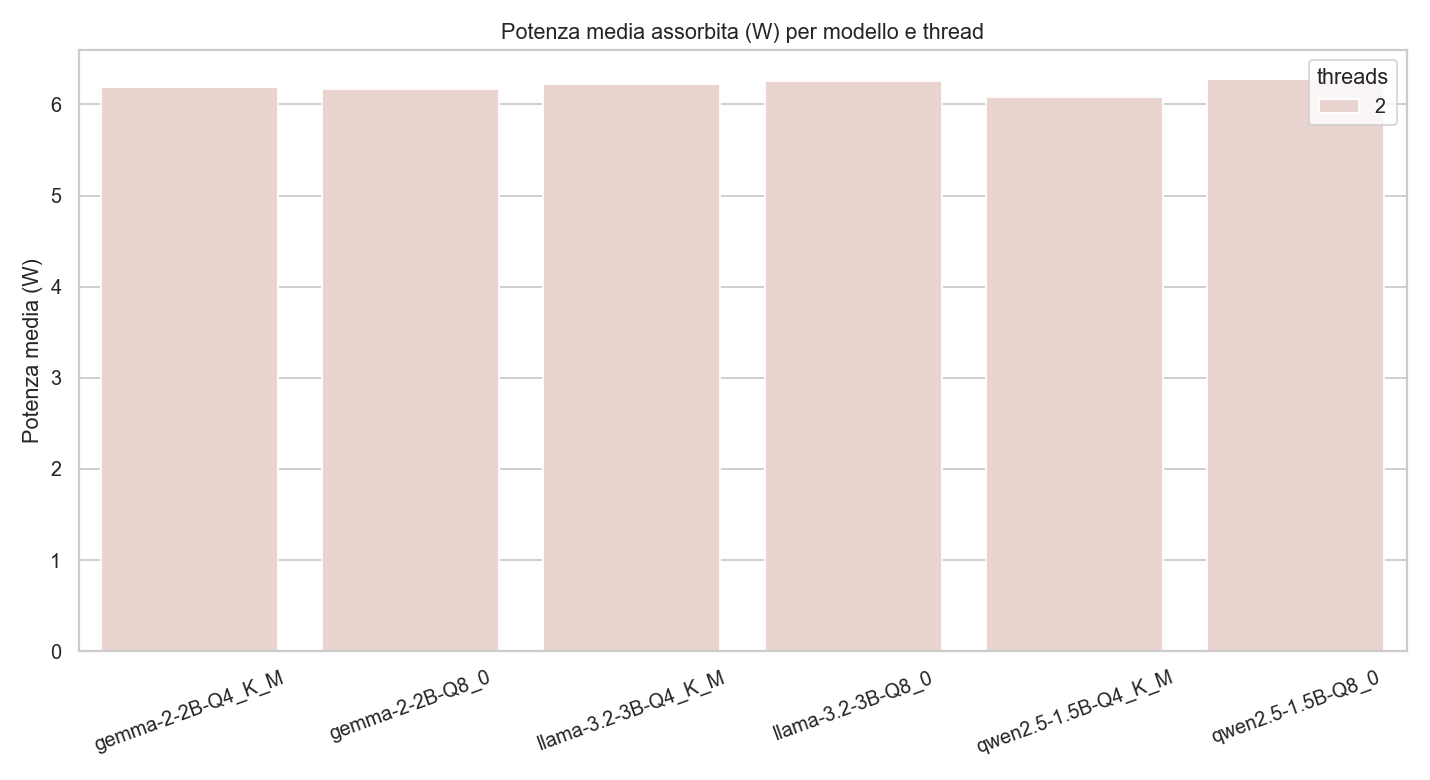
\includegraphics[width=\textwidth]{imm/power_a.png}
    \caption{Potenza media assorbita per modello, a 2 thread (Campagna A). La potenza
    è pressoché costante tra i modelli, poiché determinata dal grado di parallelismo
    più che dal modello eseguito.}
    \label{fig:res-potenza-modelli}
\end{figure}

\subsection{Qualità delle risposte}

La Figura~\ref{fig:res-qualita} mostra, sotto forma di mappa di calore, la
frazione di risposte corrette (score da 0 a 1) di ciascun modello su ciascun
benchmark. Il modello con la qualità media più elevata è \textbf{qwen2.5-1.5B
Q4\_K\_M} (accuratezza media circa \textbf{0,71}), mentre il valore più basso
spetta a \textbf{gemma-2-2B Q8\_0} (0,66); le differenze fra modelli restano
comunque contenute (tutti tra 0,66 e 0,71). A livello di singolo benchmark
emergono però specializzazioni marcate: il modello più grande, Llama-3.2-3B,
eccelle sui task di ragionamento --- BIG-Bench Hard (0,80) e GSM8K (fino a 0,80)
--- mentre i modelli più piccoli lo superano nettamente sui quesiti di senso
comune (CommonsenseQA, qwen fino a 0,77 contro circa 0,53 di llama) e sulla
generazione di codice (HumanEval, qwen fino a 0,84 contro 0,56 di llama); su
TruthfulQA i valori sono ravvicinati (gemma fino a 0,74). Riguardo all'effetto
della quantizzazione sulla qualità, il passaggio da 8 a 4 bit comporta una
differenza del tutto \textbf{trascurabile} (accuratezza media 0,68 a 8 bit contro
0,69 a 4 bit): la quantizzazione più aggressiva a 4 bit non degrada in pratica la
qualità delle risposte, pur dimezzando circa lo spazio occupato e riducendo
sensibilmente il consumo.

Occorre interpretare correttamente le differenze di accuratezza osservate a livello di
\emph{singolo benchmark}, che in alcuni casi appaiono ampie tra le due precisioni dello
stesso modello (ad esempio qwen2.5-1.5B su GSM8K: 0,57 a 4 bit contro 0,41 a 8 bit).
Esse derivano dalla combinazione di due fattori.

Il primo è che la quantizzazione produce modelli \emph{genuinamente diversi}:
arrotondando i pesi a 4 o a 8 bit si modificano leggermente le distribuzioni di
probabilità sui token. Sui prompt in cui il modello è "sicuro" il token più probabile
resta lo stesso e la risposta non cambia; sui prompt \emph{incerti}, invece, anche una
piccola perturbazione dei pesi può ribaltare l'esito. Le divergenze tra le due
precisioni si concentrano perciò sui compiti \textbf{al limite delle capacità del
modello} --- come il ragionamento aritmetico multi-passaggio di GSM8K per un modello da
appena 1,5 miliardi di parametri --- mentre sui compiti in cui il modello è a suo agio
le due precisioni coincidono quasi perfettamente (su CommonsenseQA, ad esempio,
qwen2.5-1.5B a 4 e a 8 bit ottiene risultati praticamente identici).

Il secondo fattore è che ciascun benchmark è valutato su soli \textbf{30 prompt}:
l'accuratezza di una singola cella porta quindi un'incertezza statistica dell'ordine di
$\pm 9$ punti percentuali (l'errore standard di una proporzione stimata su 30 campioni),
per cui uno scarto di cella anche ampio può non riflettere una reale differenza di
qualità. Per questi motivi la mappa di calore va letta come indicativa delle
\emph{tendenze} per singolo compito, mentre il confronto affidabile è quello condotto
sulla \textbf{media complessiva} dei 150 prompt (Figura~\ref{fig:res-qualita-media}): lì
gli intervalli di confidenza al 95\% delle due precisioni di ogni famiglia si
sovrappongono, e il verso stesso dello scarto cambia da famiglia a famiglia (8 bit
lievemente superiore per Llama-3.2-3B, 4 bit per gemma e qwen), a conferma che 4 e 8 bit
sono \textbf{sostanzialmente equivalenti} in qualità e che nessuna delle due precisioni
è sistematicamente migliore.

\begin{figure}[htbp]
    \centering
    
\includegraphics[width=\textwidth]{imm/quality_heatmap.png}
    \caption{Qualità delle risposte (accuratezza media) per modello e benchmark (Campagna A).}
    \label{fig:res-qualita}
\end{figure}

\begin{figure}[htbp]
    \centering
    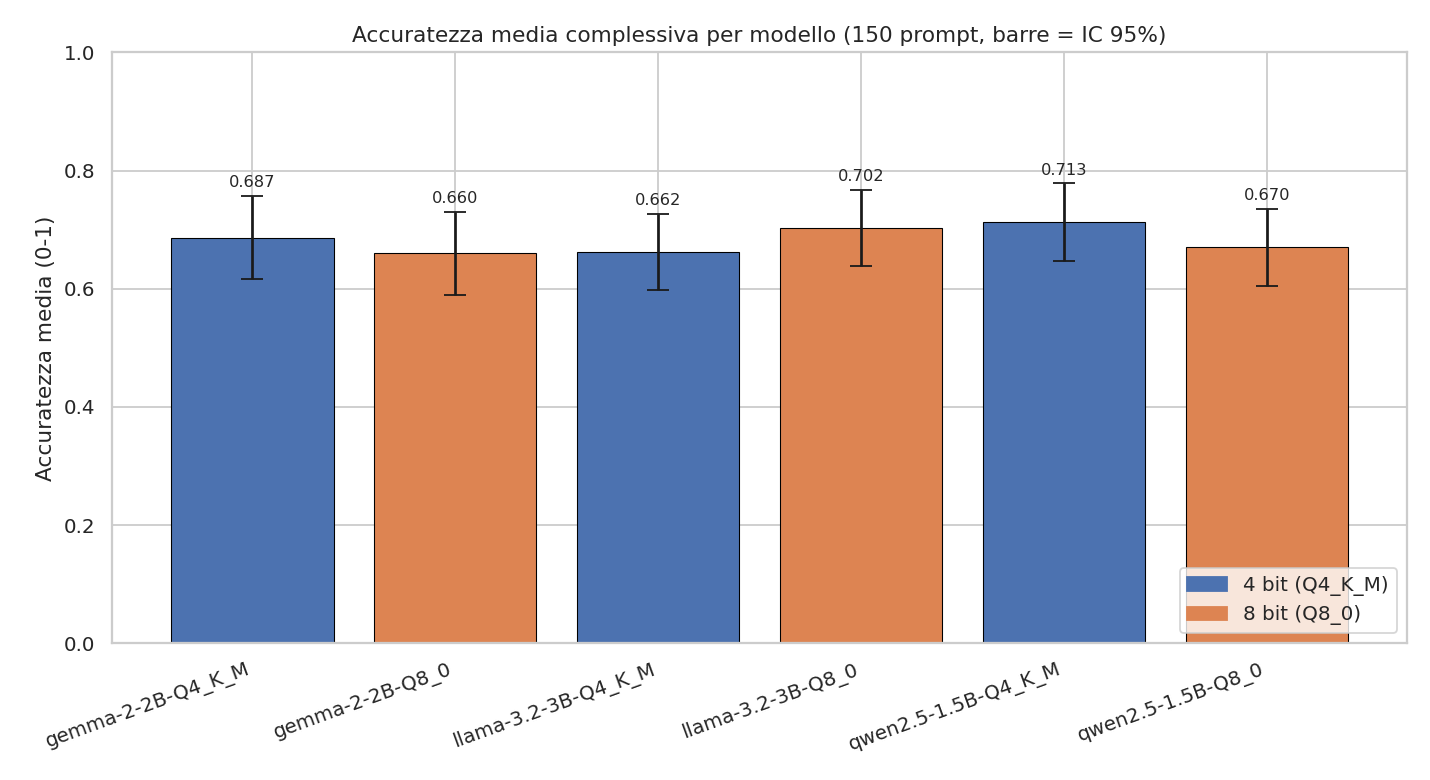
\includegraphics[width=\textwidth]{imm/quality_overall.png}
    \caption{Accuratezza media complessiva per modello (Campagna A, 150 prompt), con
    barre d'errore pari all'intervallo di confidenza al 95\%. All'interno di ogni
    famiglia gli intervalli delle due precisioni (4 e 8 bit) si sovrappongono
    ampiamente: le differenze di qualità non sono statisticamente significative.}
    \label{fig:res-qualita-media}
\end{figure}

\subsection{Velocità di elaborazione}

La Figura~\ref{fig:res-throughput} riporta la velocità di elaborazione dei prompt
(\textit{prompt processing}) e di generazione (\textit{generation}) in token al
secondo. La generazione, che determina in larga parte la latenza percepita, varia
da circa \textbf{5,1} a \textbf{17,9} token/s a seconda del modello: come atteso i
modelli più piccoli (qwen2.5-1.5B, fino a 17,9~t/s) generano molto più
rapidamente dei più grandi (Llama-3.2-3B e gemma-2-2B a 8 bit, intorno a
5,1~t/s). L'effetto della quantizzazione sulle due fasi è però \emph{opposto}. In
\textbf{generazione} --- che produce un token alla volta ed è limitata dalla
larghezza di banda della memoria --- il 4 bit è più veloce dell'8 bit (ad esempio
qwen2.5-1.5B: 17,9 contro 11,5~t/s), perché deve leggere circa metà dei byte per
token. Nel \textbf{prompt processing}, invece, i token del prompt vengono elaborati
insieme (prodotti matrice-matrice, con i pesi riutilizzati su molti token): la fase è
limitata dal \emph{calcolo} più che dalla memoria, e a pesare è il costo di
dequantizzazione dello schema a 4 bit (Q4\_K\_M, più complesso del semplice Q8\_0). Di
conseguenza è l'\textbf{8 bit} a risultare più veloce nel prompt processing
(qwen2.5-1.5B: 41,2 contro 31,8~t/s; gemma e Llama circa \mbox{+10--13\%}). Poiché
però la latenza complessiva è dominata dalla generazione (256 token prodotti a fronte
di prompt brevi), nel complesso il 4 bit resta più rapido \emph{end-to-end}.

Questo effetto si riflette direttamente sulla \textbf{latenza} di inferenza
(Figura~\ref{fig:res-latenza-modelli}). A parità
di modello e di parallelismo (2 thread), le varianti a \textbf{8 bit} risultano
mediamente circa il \textbf{30\% più lente} delle corrispondenti a 4 bit: l'aumento
va da \mbox{+13\%} per qwen2.5-1.5B (da 6,0 a 6,8~s) a \mbox{+34\%} per gemma-2-2B
(da 9,6 a 12,9~s) e \mbox{+37\%} per Llama-3.2-3B (da 12,1 a 16,5~s). La ragione è
la stessa che spiega il maggior consumo: gli 8 bit richiedono di leggere circa il
doppio dei byte per ogni token generato e, su un dispositivo limitato dalla larghezza
di banda della memoria, ciò allunga in proporzione i tempi di generazione. I 4 bit
offrono quindi, oltre a un minor consumo, anche una latenza sensibilmente inferiore.

\begin{figure}[htbp]
    \centering
    
\includegraphics[width=\textwidth]{imm/throughput.png}
    \caption{Velocità di elaborazione (prompt e generazione) per modello (Campagna A).}
    \label{fig:res-throughput}
\end{figure}

\begin{figure}[htbp]
    \centering
    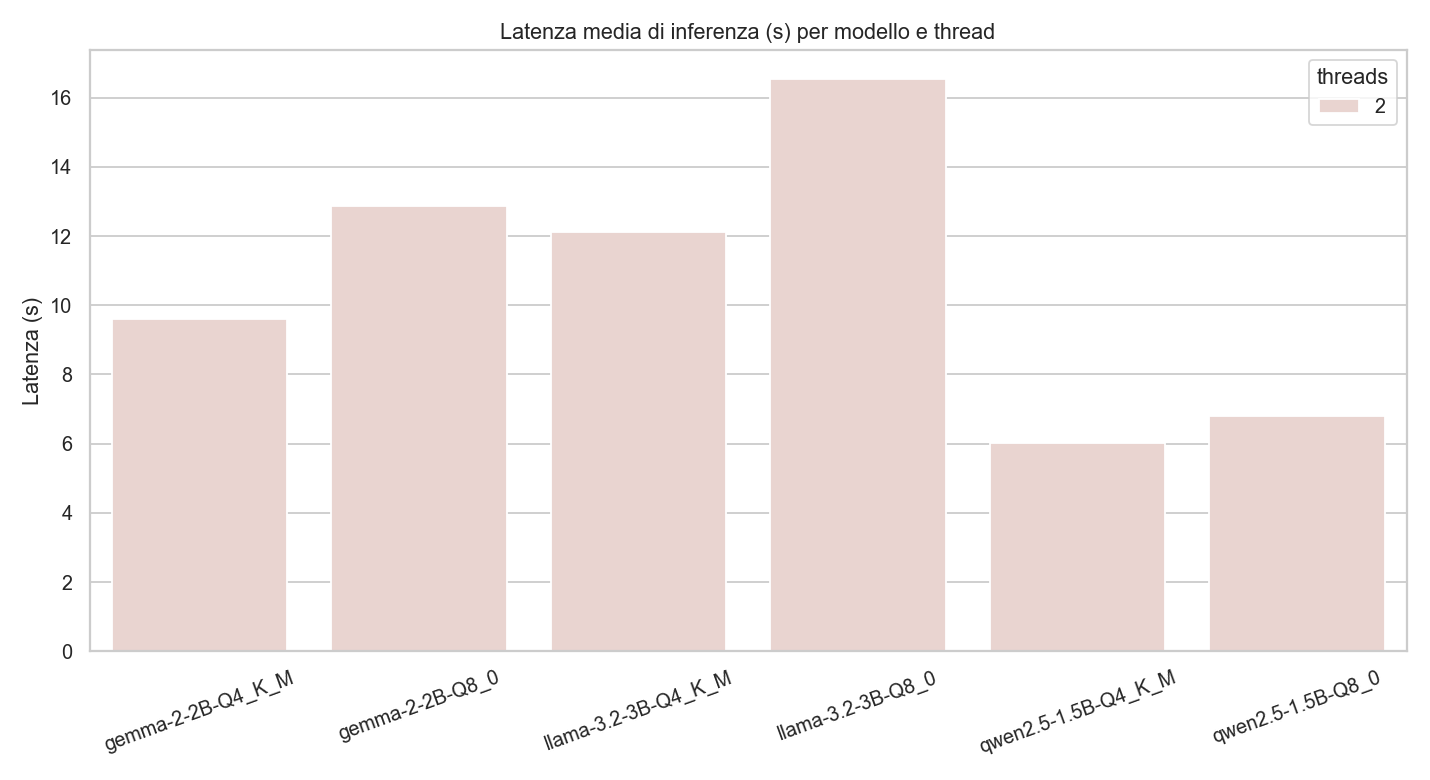
\includegraphics[width=\textwidth]{imm/latency_a.png}
    \caption{Latenza media di inferenza per modello, a 2 thread (Campagna A). A parità
    di famiglia, la variante a 8 bit (Q8\_0) presenta una latenza superiore rispetto a
    quella a 4 bit (Q4\_K\_M).}
    \label{fig:res-latenza-modelli}
\end{figure}

\section{Effetto del grado di parallelismo (Campagna B)}
\label{sec:camp-b}

Poiché il numero di thread influenza solo i tempi e i consumi dell'inferenza e
non le risposte generate dal modello, in questa campagna la qualità non viene
ridiscussa: essa è stata misurata in modo robusto nella Campagna A. Qui
l'attenzione è rivolta all'effetto del parallelismo su latenza, potenza ed
energia.

\subsection{Latenza}

La Figura~\ref{fig:res-latenza} mostra la latenza media di inferenza al variare
del numero di thread (1, 2 e 4). Passando da 1 a 2 thread la latenza si riduce di
circa \textbf{24\%} (da 14,2 a 10,9~s in media), mentre l'ulteriore passaggio da 2
a 4 thread non porta alcun guadagno --- anzi la latenza \emph{peggiora}
(circa \mbox{+18\%}, risalendo a 12,8~s). Diversi benchmark sono limitati dalla
larghezza di banda della memoria più che dal numero di core: il terzo e quarto core
non accelerano la generazione e introducono contesa. Il valore ottimale di
parallelismo risulta quindi \textbf{2 thread}.

Un dettaglio interessante riguarda il confronto tra le due precisioni \emph{a 1 thread}:
per ogni modello la latenza è più bassa con la variante a \textbf{8 bit} che con quella a
4 bit (ad esempio qwen2.5-1.5B: 7,6~s contro 9,6~s), in apparente contrasto con il fatto
che i 4 bit debbano leggere meno dati. La spiegazione è ancora la distinzione tra carico
limitato dalla \emph{memoria} e carico limitato dal \emph{calcolo}. Con un solo thread il
bus di memoria non è saturo, quindi anche la generazione è più \emph{compute-bound} che
\emph{memory-bound}: in questo regime il vantaggio del 4 bit (metà dei byte da leggere) è
annullato dal suo maggior costo di \textbf{dequantizzazione} (lo schema Q4\_K\_M è più
complesso del semplice Q8\_0), tanto che la velocità di generazione delle due precisioni
diventa praticamente identica (a 1 thread circa 7,7~t/s per il 4 bit contro 7,5~t/s per
l'8 bit). A ciò si aggiunge la fase di \emph{prompt processing}, anch'essa compute-bound e
più rapida a 8 bit: il risultato netto è una latenza complessiva inferiore per l'8 bit a
1 thread. Passando a 2 o 4 thread, invece, i core saturano la banda di memoria e la
generazione torna \emph{memory-bound}: il 4 bit riprende un netto vantaggio (a 2 thread
11,5 contro 7,4~t/s) e, poiché la generazione domina la latenza complessiva, è di nuovo
il 4 bit ad avere la latenza più bassa.

\begin{figure}[htbp]
    \centering
    
\includegraphics[width=\textwidth]{imm/latency.png}
    \caption{Latenza media di inferenza al variare del numero di thread (Campagna B).}
    \label{fig:res-latenza}
\end{figure}

\subsection{Potenza ed energia}

All'aumentare del numero di thread la potenza media assorbita \textbf{cresce}
(da circa 4,9~W a 1 thread a 7,0~W a 4 thread, Figura~\ref{fig:res-potenza}).
L'energia netta per inferenza è \textbf{minima a 1 thread} (circa 40,6~J) e cresce
con il parallelismo: solo lievemente da 1 a 2 thread (\mbox{+10\%}, circa 44,8~J),
ma nettamente a 4 thread (\mbox{+28\%} rispetto a 2 thread, circa 57,5~J). In
termini di sola energia il minimo si ha quindi a 1 thread, ma a fronte di una
latenza molto più elevata; il miglior compromesso tra \textit{time-to-answer} ed
efficienza energetica è a \textbf{2 thread}, che riduce di circa un quarto la
latenza con un modesto sovrapprezzo energetico, mentre a 4 thread si perde su
entrambi i fronti.

Un dettaglio degno di nota riguarda il confronto tra le due precisioni al variare del
parallelismo: la potenza media delle varianti a 4 e a 8 bit si \emph{ribalta} passando
da 1 a 4 thread. A \textbf{1 thread} le varianti a 8 bit assorbono circa 0,4~W in più
delle corrispondenti a 4 bit, mentre a \textbf{4 thread} sono queste ultime a consumare
di più (circa 0,65~W in più) --- e il comportamento è uniforme in tutte e tre le
famiglie. A prima vista il risultato sorprende --- il modello a 4 bit, più leggero, dovrebbe
consumare sempre meno --- ma si spiega ricordando che la potenza istantanea misura
\emph{quanto i core stanno effettivamente calcolando}, e non la quantità totale di
lavoro da svolgere: un core che calcola assorbe potenza, mentre un core fermo in
\emph{stallo} ad attendere i dati dalla memoria ne assorbe molta meno. Poiché il
carico è limitato dalla \textbf{larghezza di banda della memoria}, è proprio la quota
di tempo che i core trascorrono in stallo a determinare il ribaltamento. Con un solo thread il bus di memoria non è saturo e il modello a 8 bit
--- che deve leggere circa il doppio dei byte per token --- tiene il core più occupato,
assorbendo un po' di più. Con quattro thread, invece, i core competono per la stessa
banda condivisa: il modello a 8 bit la satura e i core trascorrono più tempo in stallo
(un core fermo consuma meno), mentre il modello a 4 bit, più leggero, li mantiene
attivi nel calcolo, assorbendo così una potenza maggiore. Questo \emph{non} penalizza i
4 bit: la potenza aggiuntiva si traduce in calcolo utile, tant'è che a 4 thread le
varianti a 4 bit restano più veloci (latenza media 10,0~s contro 15,5~s) e più
efficienti (47,7~J contro 67,4~J per inferenza).

Va precisato che questa spiegazione, per quanto coerente con i dati e con la natura
\emph{memory-bandwidth bound} del carico, resta un'\textbf{interpretazione}: le misure
disponibili registrano la sola potenza \emph{complessiva} della scheda (la somma dei
dodici rami del PMIC), non l'andamento dei singoli rami. Una dimostrazione diretta
richiederebbe di visualizzare separatamente i \textbf{dodici canali del PMIC} --- in
particolare confrontando i rami della memoria (\textit{DDR\_VDD2}, \textit{DDR\_VDDQ})
con quello del core del SoC (\textit{VDD\_CORE}) --- così da osservare l'effettivo
spostamento del consumo tra sottosistema di memoria e sottosistema di calcolo al
variare del grado di parallelismo.

\begin{figure}[htbp]
    \centering
    
\includegraphics[width=\textwidth]{imm/power.png}
    \caption{Potenza media assorbita al variare del numero di thread (Campagna B).}
    \label{fig:res-potenza}
\end{figure}

\section{Frontiere di Pareto}

Per individuare le configurazioni migliori senza fissare a priori un peso relativo tra
gli obiettivi si ricorre al concetto di \emph{frontiera di Pareto}: una configurazione
si dice \emph{dominata} se ne esiste un'altra migliore (o uguale) su entrambi gli
obiettivi considerati, e strettamente migliore su almeno uno; le configurazioni
\emph{non dominate} costituiscono la frontiera, cioè l'insieme dei compromessi ottimali
per cui non è possibile migliorare un obiettivo senza peggiorare l'altro. A differenza
dello score composito, questa rappresentazione non richiede la scelta di pesi: evidenzia
direttamente i candidati razionali e lascia al lettore la decisione finale in base alle
proprie priorità. Il criterio si applica sia al confronto tra i modelli (Campagna A) sia
alla scelta del grado di parallelismo (Campagna B).

\subsection{Confronto tra i modelli (Campagna A)}

La Figura~\ref{fig:res-pareto-en} riporta la frontiera nel piano
\textbf{energia--qualità} (le configurazioni in basso a destra sono le migliori). Il
risultato è particolarmente netto: \textbf{qwen2.5-1.5B Q4\_K\_M} unisce l'energia
minima (24,6~J) a una qualità tra le più elevate; poiché nessun'altra configurazione la
supera contemporaneamente su entrambi gli assi, essa risulta l'unico punto \emph{non
dominato} della frontiera. Va però ricordato che le differenze di qualità tra i modelli
di testa rientrano nella variabilità di misura, per cui questa posizione dominante è
trainata soprattutto dal consumo nettamente inferiore di qwen a 4 bit. Le configurazioni
Llama-3.2-3B, in particolare, risultano nettamente \emph{dominate}. La
Figura~\ref{fig:res-pareto-lat} mostra l'analoga frontiera nel piano
\textbf{latenza--qualità}, sempre per i sei modelli a 2 thread.

\begin{figure}[htbp]
    \centering
    
\includegraphics[width=\textwidth]{imm/pareto_energia.png}
    \caption{Frontiera di Pareto nel piano energia--qualità (Campagna A, i sei modelli a 2 thread; cerchiate in rosso le configurazioni non dominate).}
    \label{fig:res-pareto-en}
\end{figure}

\begin{figure}[htbp]
    \centering
    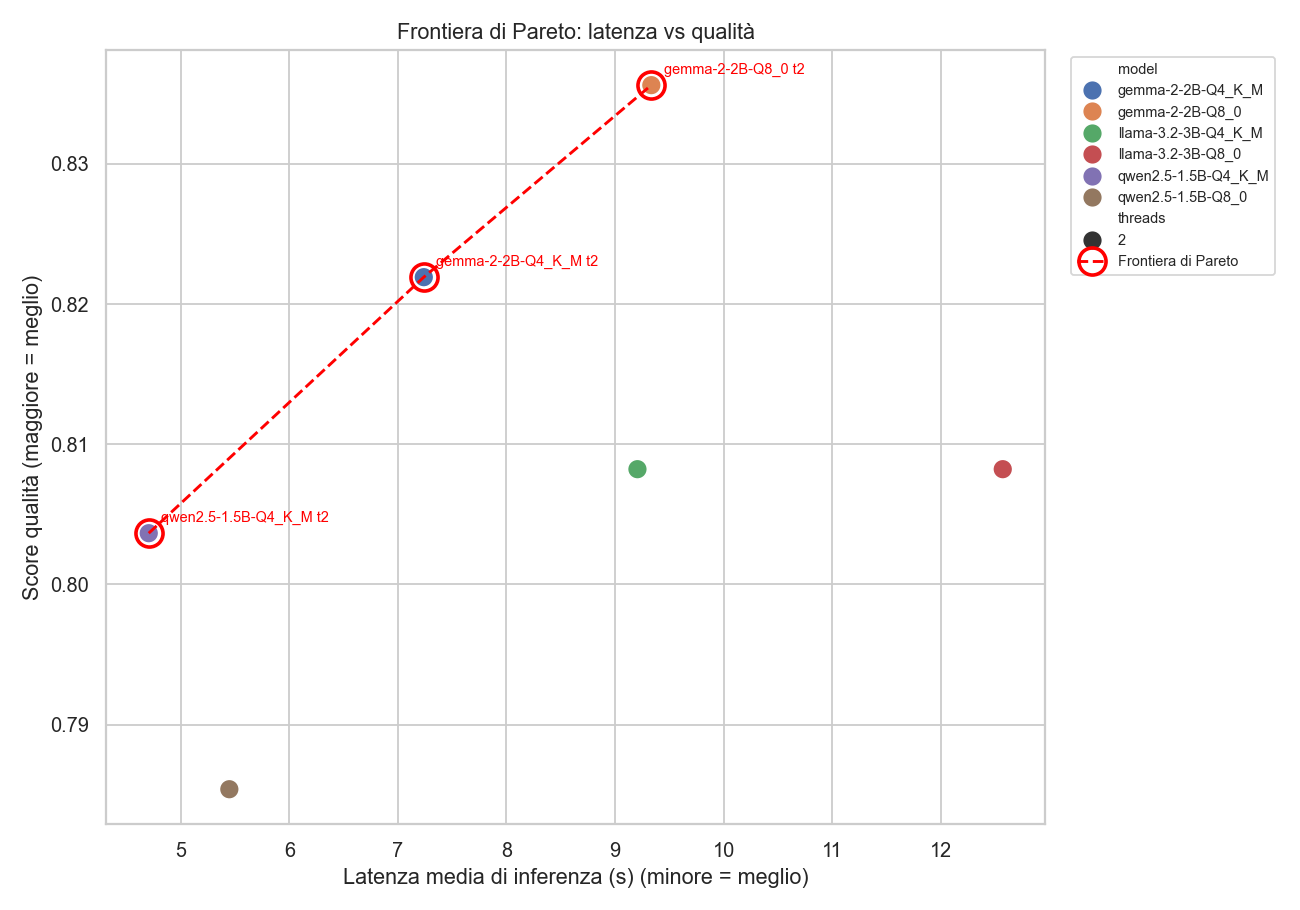
\includegraphics[width=\textwidth]{imm/pareto_latenza.png}
    \caption{Frontiera di Pareto nel piano latenza--qualità (Campagna A, i sei modelli a 2 thread).}
    \label{fig:res-pareto-lat}
\end{figure}

\subsection{Scelta del grado di parallelismo (Campagna B)}

Nella Campagna B la qualità non entra in gioco (il numero di thread non cambia le
risposte): latenza ed energia sono due \emph{costi} che il parallelismo influenza in
direzioni potenzialmente opposte. Rappresentando ciascuna configurazione nel piano
\textbf{latenza--energia} si individuano, per ogni modello, le combinazioni di thread
\emph{non dominate}. La Figura~\ref{fig:res-pareto-thread} riporta, per i sei modelli,
la traiettoria al variare dei thread (1, 2 e 4) e marca in rosso le configurazioni
dominate. Il risultato è netto: la configurazione a \textbf{4 thread è dominata in
cinque modelli su sei}, perché rispetto ai 2 thread consuma di più senza ridurre la
latenza (anzi spesso aumentandola); l'unica eccezione è qwen2.5-1.5B Q4\_K\_M, mentre per
Llama-3.2-3B Q4\_K\_M la dominanza è ancora più forte (risultano dominati sia 1 sia 4
thread, e l'unico punto sulla frontiera è quello a 2 thread). La frontiera di ciascun
modello si riduce così ai soli 1 e 2 thread: la scelta razionale è tra \textbf{1 thread}
(energia minima, ma latenza elevata) e \textbf{2 thread} (latenza minima, con un modesto
sovrapprezzo energetico), mentre i 4 thread quasi mai rappresentano un compromesso
ottimale --- una conferma \emph{senza pesi} dei 2 thread come miglior compromesso.

\begin{figure}[htbp]
    \centering
    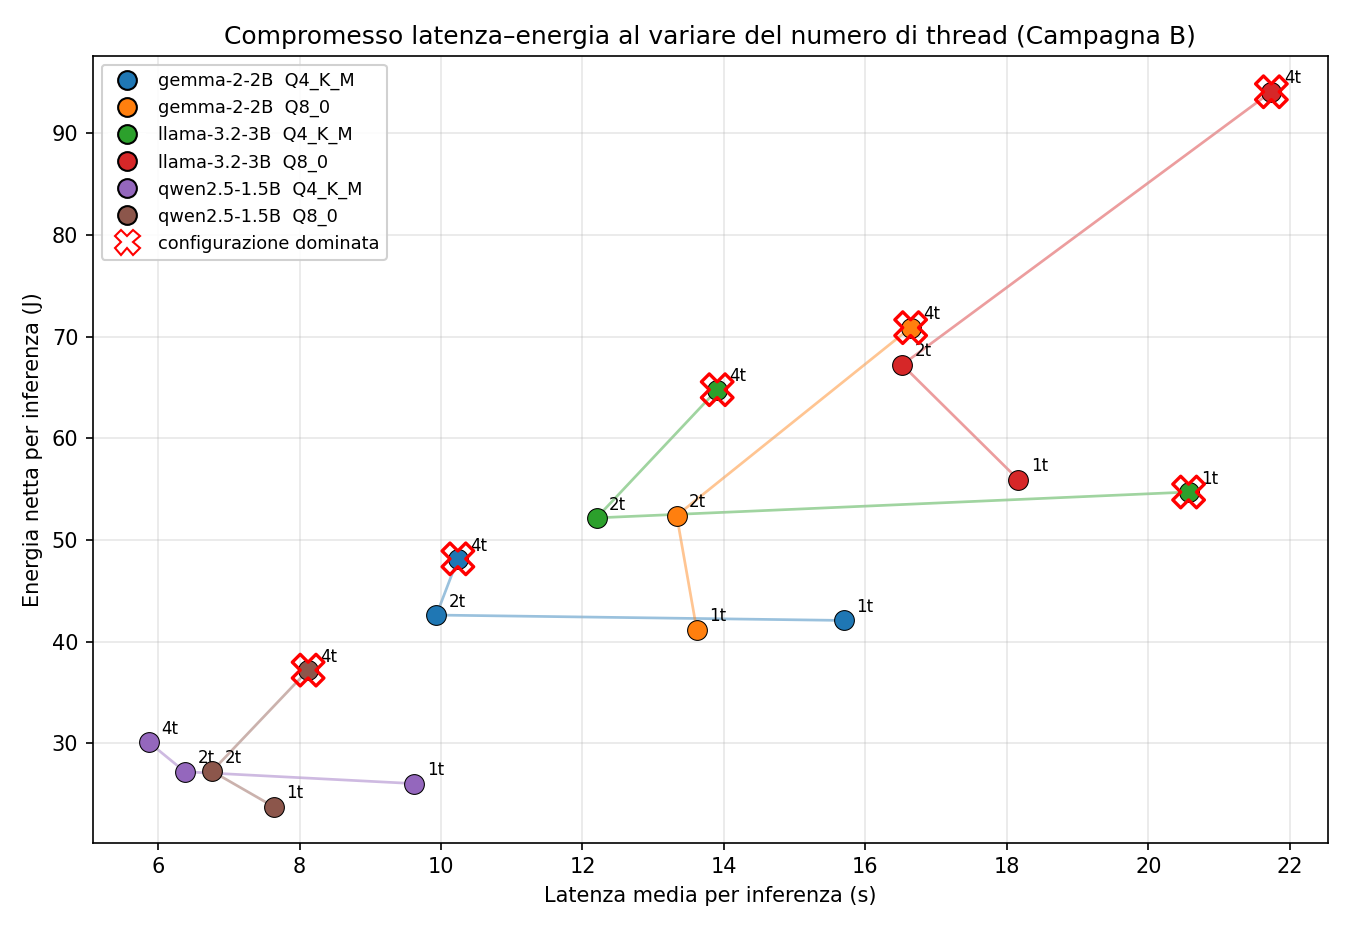
\includegraphics[width=\textwidth]{imm/pareto_lat_energia.png}
    \caption{Compromesso latenza--energia al variare del numero di thread (Campagna B):
    per ogni modello è tracciata la traiettoria a 1, 2 e 4 thread e sono marcate in rosso
    le configurazioni dominate. I 4 thread risultano dominati in cinque modelli su sei.}
    \label{fig:res-pareto-thread}
\end{figure}

\section{Sintesi: classifica complessiva}
\label{sec:composito}

Per riassumere in un unico indicatore le tre dimensioni di analisi si definisce uno
\emph{score composito}. Le tre metriche di una configurazione --- energia netta per
inferenza $E$, latenza $L$ e accuratezza media $Q$ --- hanno unità di misura e
intervalli di valori diversi; per renderle confrontabili vengono normalizzate con
una trasformazione \emph{min--max} sull'insieme delle configurazioni:
\begin{equation}
    \tilde{x} = \frac{x - x_{\min}}{x_{\max} - x_{\min}} \in [0, 1],
    \label{eq:minmax}
\end{equation}
dove $x_{\min}$ e $x_{\max}$ sono il valore minimo e massimo di quella metrica tra
tutte le configurazioni confrontate. Poiché per l'energia e la latenza sono
preferibili valori \emph{bassi}, mentre per la qualità è preferibile un valore
\emph{alto}, lo score composito $C$ è definito come media pesata in cui i termini
di energia e latenza vengono invertiti:
\begin{equation}
    C = w_E\,(1 - \tilde{E}) + w_L\,(1 - \tilde{L}) + w_Q\,\tilde{Q},
    \qquad w_E + w_L + w_Q = 1,
    \label{eq:composito}
\end{equation}
con pesi $w_E = 0{,}4$ (energia), $w_L = 0{,}2$ (latenza) e $w_Q = 0{,}4$
(qualità). A un valore di $C$ più alto corrisponde una configurazione
complessivamente migliore.

La scelta dei pesi riflette le priorità dello studio: l'\emph{efficienza
energetica} e la \emph{qualità delle risposte} sono considerate gli obiettivi
primari e ricevono quindi lo stesso peso ($0{,}4$ ciascuno), mentre alla
\emph{latenza} è attribuito un peso inferiore ($0{,}2$), essendo un requisito meno
stringente per molte applicazioni edge non strettamente interattive. Trattandosi
di una scelta soggettiva, lo score composito va inteso come una sintesi
orientativa e non come un giudizio assoluto: per questo motivo è affiancato dalla
frontiera di Pareto (Figure~\ref{fig:res-pareto-en} e~\ref{fig:res-pareto-lat}),
che individua le configurazioni ottimali \emph{senza} richiedere alcuna scelta di
pesi.

Lo score è calcolato sulle sei configurazioni della \textbf{Campagna A} (i sei
modelli a 2 thread), coerentemente con l'obiettivo di confrontare i modelli a parità
di grado di parallelismo. La Figura~\ref{fig:res-composito} riporta la relativa
classifica. La configurazione complessivamente migliore risulta
\textbf{qwen2.5-1.5B Q4\_K\_M a 2 thread} (score \textbf{1,00}), seguita da
\textbf{qwen2.5-1.5B Q8\_0} (0,67) e \textbf{gemma-2-2B Q4\_K\_M} (0,59): qwen a 4
bit ottiene il punteggio massimo perché unisce l'energia più bassa e la latenza più
bassa a una qualità competitiva --- il primato è trainato soprattutto dai vantaggi,
robusti, su energia e latenza, dato che le differenze di qualità tra i modelli di
testa rientrano nel rumore di misura ---, mentre le configurazioni Llama-3.2-3B,
penalizzate da consumo ed energia
elevati, si collocano in fondo alla classifica nonostante la buona qualità sui
task di ragionamento.

\begin{figure}[htbp]
    \centering
    
\includegraphics[width=\textwidth]{imm/ranking_composite.png}
    \caption{Classifica complessiva dei sei modelli secondo lo score composito
    (Campagna A, a 2 thread).}
    \label{fig:res-composito}
\end{figure}

\section{Comportamento termico}

Durante entrambe le campagne la temperatura del SoC è stata monitorata dopo ogni
inferenza. Grazie alla ventola di raffreddamento attiva --- e, nella Campagna B,
alle pause di raffreddamento tra le configurazioni --- la temperatura si è mantenuta
sotto la soglia di \textit{throttling} ($\sim$80--85~\textcelsius): nella Campagna A
(2 thread) il massimo è stato di \textbf{76,8}~\textcelsius, mentre nella Campagna B
i picchi si sono avuti sulle configurazioni a 4 thread, comunque contenuti intorno
agli \textbf{81}~\textcelsius\ (Figura~\ref{fig:res-termico}). In \textbf{nessuna}
delle due campagne si è verificato throttling, per cui le misure di latenza ed
energia non sono state falsate da riduzioni di frequenza indotte dal calore. Poiché in
entrambe le campagne il funzionamento è avvenuto a piena frequenza, le misure
restano inoltre \emph{direttamente confrontabili}, nonostante la Campagna B adotti
le pause di raffreddamento assenti nella Campagna A: la pausa agisce solo sulla
temperatura di picco, che al di sotto della soglia di throttling non influenza né la
latenza né l'energia.

Va tuttavia osservato che sessioni di misura molto prolungate, sommando il
riscaldamento del SoC alla sollecitazione continua in lettura della scheda microSD,
possono compromettere l'integrità dei file dei modelli memorizzati; per questo
motivo la procedura adotta la verifica di integrità all'avvio e le pause di
raffreddamento descritte nel capitolo precedente.

\begin{figure}[htbp]
    \centering
    
\includegraphics[width=\textwidth]{imm/thermal.png}
    \caption{Distribuzione della temperatura del SoC durante le inferenze della
    Campagna B, che comprende le configurazioni a 4 thread, termicamente più
    impegnative.}
    \label{fig:res-termico}
\end{figure}

\chapter{Conclusioni}

In questo capitolo vengono riassunti i risultati ottenuti e le conclusioni
tratte dallo studio condotto. Si evidenziano le principali scoperte, le implicazioni
dei risultati e le possibili direzioni future per ulteriori ricerche o applicazioni pratiche.

%\chapter{Ringraziamenti}

Grazie a tutti fratelli.
Pace e amore, baci e abbracci a tutti.


\bibliographystyle{plain}
\nocite{*}
\bibliography{bibliografia}


\end{document}
